\documentclass[11pt,a4paper,oneside]{report}
\usepackage[margin=22mm]{geometry}
\usepackage[T1]{fontenc}
\usepackage{lmodern,microtype,amsmath,amssymb,booktabs,longtable,array,graphicx,xcolor,caption}
\usepackage[unicode,colorlinks=true,linkcolor=blue!55!black,urlcolor=blue!55!black,bookmarksnumbered]{hyperref}
\usepackage{fancyhdr}
\usepackage{titlesec}
\titleformat{\chapter}[display]{\normalfont\bfseries}{\large\chaptertitlename\ \thechapter}{8pt}{\LARGE}
\titlespacing*{\chapter}{0pt}{0pt}{18pt}
\pagestyle{fancy}\fancyhf{}\fancyhead[L]{\small ACE: October 25 research record}\fancyhead[R]{\small Pre-golden study}\fancyfoot[C]{\thepage}
\setlength{\headheight}{14pt}
\setlength{\parindent}{0pt}\setlength{\parskip}{6pt}
\setlength{\emergencystretch}{1em}
\setlength{\LTpre}{5pt}\setlength{\LTpost}{5pt}
\setlength{\tabcolsep}{4pt}\renewcommand{\arraystretch}{1.15}
\hypersetup{pdftitle={ACE routing and Dynamic preparation: October 25 pre-golden-study report},pdfauthor={Compiler-Driven-ACE project}}
\newcommand{\repo}{https://github.com/sanjeevkrishnaa/Compiler-Driven-ACE}
\newcommand{\snap}{4aa334542e9b9c8fe7a5f9cc8fe48ee2e4d2fa55}
\newcommand{\src}[2]{\href{\repo/blob/\snap/#1}{#2}}
\newcommand{\commit}[1]{\href{\repo/commit/#1}{\texttt{#1}}}
\begin{document}
\hypersetup{pageanchor=false}
\begin{titlepage}
\centering\vspace*{25mm}
{\Large Compiler-Driven ACE\par}\vspace{12mm}
{\Huge\bfseries Routing, congestion and Dynamic EPR preparation\par}
\vspace{12mm}{\LARGE Research record for 25 October 2026\par}
\vspace{8mm}{\large A fresh retrospective of the experiments before the golden study\par}
\vfill
\begin{minipage}{.88\textwidth}
This report reconstructs the archived experimental evidence from a fixed Git snapshot. It explains the model, timing corrections, routing alternatives, preparation rules, successful results and unsuccessful trials. Every research figure is followed by its numerical table and a CSV link. The October 26 golden-study results are outside this report's scope.

Evidence boundary: \commit{4aa3345}, immediately before the first golden-study commit \commit{44fa139}. Prepared on 26 October 2026 (IST).
\end{minipage}\vspace{18mm}
\end{titlepage}
\hypersetup{pageanchor=true}\pagenumbering{roman}\tableofcontents\clearpage\pagenumbering{arabic}

\chapter{Purpose, scope and the principal result}
The question studied on October 25 was why compiler-driven pre-generation could lose to on-demand generation (ODG), and whether changing routes or the choice of hops to prepare could recover the benefit. The evidence supports a conditional answer: early EPR generation saves service time, but cached pairs occupy shared communication memories. Contention can cost more time than pre-generation saves. Changing routing and reducing unnecessary later-hop preparation can reduce that cost.

The corrected reference uses the supplied QFT-96 trace on a $4\times4$ mesh, four shared communication memories per core, at most three compiler-held memories per core, and 30 physics seeds. Full-chain Dynamic has mean request latency $2.570$ ms versus ODG's $1.526$ ms. Replacing the supplied routes with XY reduces full-chain Dynamic to $1.484$ ms, while ODG itself improves to $1.340$ ms. Thus routing alone helps substantially but does not make full-chain Dynamic beat the same-route ODG on mean latency.

First-hop-only preparation on XY reaches $1.194$ ms. A congestion-adaptive rule selected using a layer-activity screen reaches $1.175$ ms in the 30-seed confirmation. Against XY's own ODG reference, that is approximately $12.3\%$ lower latency and $5.9\%$ shorter communication makespan. These results apply to this archived model and workload. The threshold was selected on QFT-96; the 30-seed confirmation repeats the screening seeds and adds further seeds, so it is not a wholly held-out confirmation.

The ten-workload tests also show why a universal victory claim would be wrong. They use \emph{48-qubit} circuits and only three physics seeds per cell. Full-chain Dynamic is already strong on several sparse workloads. First-hop-only can sacrifice that advantage. The adaptive threshold retains full-chain behaviour on many of them, but does not outperform every alternative on every workload.

\section{How to read this report}
Chapters 2--3 establish the model and historical timing context. Chapters 4--8 follow the routing and preparation experiments in their logical order. Chapter 9 records the generalisation tests. Chapter 10 explains the separate HQA/T-HQA comparison and newly implemented controls. The appendices give commit links, reproducibility instructions and the data index.

\section{Evidence boundary}
The snapshot is \texttt{4aa3345}, the parent of \texttt{44fa139}, where the golden-study contract begins. A Git boundary is more reliable than sorting author timestamps: merged work and rewritten messages do not necessarily appear in timestamp order. Tables are regenerated by reading files directly from this Git revision; later modifications to working-tree result files cannot alter this retrospective.

The detailed routing, launch-policy, intervention, first-hop, parameter and adaptive experiments are included. Earlier October 24 experiments appear only as historical motivation. The later golden study, new T-HQA campaign, October 26 QFT chapter, QPE extension and exhaustive topology/memory matrix are excluded. CGP/ACGP results from those later campaigns must not be inserted into the October 25 two-policy comparisons.

\begin{center}\small
\begin{longtable}{lrr}
\caption{Evidence inventory. The reference family deliberately duplicates the supplied-route control for regression validation.}\\
\toprule
Family & Policy cells & Seed rows \\
\midrule\endfirsthead
\toprule
Family & Policy cells & Seed rows \\
\midrule\endhead
routing & 10 & 300 \\
reference & 2 & 60 \\
launch-screen & 26 & 260 \\
route-intervention & 32 & 960 \\
confirmation & 6 & 180 \\
threshold-screen & 10 & 100 \\
parameter-screen & 11 & 110 \\
generalisation & 60 & 180 \\
generalisation-adaptive & 20 & 60 \\
\bottomrule\end{longtable}\end{center}
{\footnotesize \href{https://github.com/sanjeevkrishnaa/Compiler-Driven-ACE/blob/codex/ace-scheduler-correctness/docs/latex/oct25_pre_golden/data/all_metrics.csv}{Complete CSV: all\_metrics}. }


\chapter{What the implementation actually measures}
\section{The simulation pipeline}
The mapper assigns qubits to cores over layers. A logical migration is $(\ell,q,s,d)$: a layer, a qubit, its source core and its destination core. A routing policy expands the migration into a physical core path. That path is expanded into adjacent-hop EPR requests, which ACE serves using the selected EPR generation policy and SeQUeNCe's discrete-event simulation.

For example, $(q,0,2)$ may become the path $0\to1\to2$, then two requests. The per-qubit scheduler preserves their order: the second hop becomes eligible after the first finishes. Different qubits in an active layer may request EPR pairs concurrently. The work studied here compares adjacent-hop EPR \emph{delivery}, not a complete physical simulation of every gate and teleported data state.

The project uses SeQUeNCe as the event engine and physical-protocol dependency; it does not execute the quantum algorithm on local quantum hardware. Time is represented internally in picoseconds. Reporting a result in milliseconds is a unit conversion, not evidence of millisecond event resolution. The magnitude of the result follows the chosen model parameters, including control delays and generation times.

\section{Memories and reservations}
Four shared communication memories per core are the reference capacity $M=4$. The compiler may occupy at most $C=3$ for prepared pairs. These are not seven separate slots. A prepared EPR half occupies a communication memory until it is used, expires or is released. The remaining capacity protects demand service, but does not guarantee that every request immediately finds a free reservation slot.

In this ACE path a request still needs admission even if a cached pair exists. The implementation transfers a usable cached pair into a request's reservation resource. Consequently, a ready pair can coexist with a waiting request. This is why readiness and latency must both be measured.

\section{The latency contract}
For a completed hop request $i$, let $a_i$ be eligibility and $c_i$ delivery:
\[
 L_i=c_i-a_i,\qquad \overline L=\frac{1}{N}\sum_{i=1}^N L_i.
\]
The first hop's eligibility is layer activation; a later hop's eligibility is predecessor completion. The interval includes shared-memory admission waiting, required control exchange, retries and EPR generation. A pair's storage before request eligibility is not added to that request's latency. It can still affect latency indirectly by blocking memories and can reduce fidelity.

Parallelism changes the set of eligibility times, not this definition. Adding the latencies of parallel requests does not yield elapsed trace time. Communication makespan is the simulated workload interval to final delivery, and includes layer progression and configured gaps. It is not the wall-clock runtime of the Python process, nor the full QFT algorithm execution time including unmodelled gates.

\section{Other metrics and their denominators}
\begin{longtable}{p{.27\linewidth}p{.65\linewidth}}
\toprule Metric & Definition and interpretation\\\midrule\endhead
Mean, median, p95, maximum & Distribution of eligible-to-delivery hop latency within each run. Reported means of per-run p95 values are not the pooled percentile of all seeds.\\
Admission wait & Time spent in the event scheduler's explicit waiting state before admission. The polling path has a different accounting mechanism; a reported zero is not proof of zero waiting.\\
Generation/service & The runner's entanglement-generation/service timing after admission. Keep this separate from queueing and control overhead; not every aggregate subcounter is an exact latency decomposition.\\
Readiness fraction & \texttt{pregenerated\_success\_rate}: distinct completed requests served by a pair physically created before first application submission, divided by all requests. This boundary is application submission, not eligibility.\\
Intended-hit rate & Requests served by the pair planned for that request, divided by all requests. It can include late use, so it is not identical to readiness.\\
Fallback fraction & Requests not served by a compiler pair divided by all requests. A compiler pair can be late without being a fallback.\\
Compiler waste & $100\,(N_{expired}+N_{remaining})/N_{generated}$, using the compiler's pair records at workload stop. Unused remaining pairs may be reusable beyond the observed horizon.\\
Compiler expiry & $100\,N_{expired}/N_{generated}$. A component of waste, not the same quantity.\\
Protocol waste & A separate native-protocol counter with different accounting. It must not replace compiler waste; the two counters are not additive.\\
Storage time & Mean generation-to-utilisation interval among used compiler pairs only. Excludes unused/expired pairs, so is conditional on use.\\
Delivered fidelity & The runner's mean fidelity of delivered EPR pairs across completed requests. This is not final QFT output-state fidelity or algorithm success probability.\\
Fidelity at use & Fidelity among utilised compiler pairs, with a different population from all delivered pairs.\\
Completion & Completed adjacent-hop requests divided by requested adjacent-hop requests. All result cells included here must pass completion validation.\\
\bottomrule
\end{longtable}
Definitions are checked against \src{compiler\_scheduler.py}{the compiler controller}, \src{run\_trace\_comparison.py}{the comparison runner}, and \src{parallel\_core.py}{the parallel engine} at the frozen snapshot. The unified per-seed CSV preserves all recorded counters, including metrics not plotted in the main text.

\section{Statistics and limits of the seeds}
Each table uses the arithmetic mean and sample SD of run-level measurements. The statistical unit is a physics-seed run, not an individual hop. These seed distributions quantify stochastic variation conditional on a fixed trace; they do not quantify variation over independent circuits or placements. The same seed number across different routes need not correspond to identical random physical events, so the archived comparison uses independent-sample Welch comparisons. The supplementary CSV retains exploratory unadjusted Welch $p$-values; many hypotheses and thresholds were tried, so these are not multiplicity-corrected confirmatory tests.

\chapter{Why the earlier midterm and corrected timings differ}
\section{The two independent changes}
The timing matrix crosses the old core/batch release scheduler with the corrected per-qubit release scheduler, and crosses a fixed 5.3 ms reservation lead with derived physical timing. These changes must be distinguished. The old local/service latency starts only when the serialized manager submits a request. It omits earlier waiting for the batch. The corrected headline starts when that request becomes eligible.

The original ACE import \commit{c29d5e6} contained the fixed \texttt{pregeneration\_time\_ms = 5.3} setting. It was an experimental pre-generation buffer, not a value derived from light travel, coherence or a physical paper constant. The historical path added it before reservation windows and removed it in the local reported number. Corrected headline runs use zero artificial lead and retain the RSVP control guard derived from configured classical delay, approximately 0.2 ms in the reference case.

\begin{center}\small
\begin{tabular}{p{.31\linewidth}rrr}
\toprule Model and metric & ODG ms & Dynamic ms & ODG/Dynamic s\\\midrule
Legacy, 5.3 ms lead; historical local & $1.110\pm.011$ & $.691\pm.008$ & $32.900/30.932$\\
Legacy, corrected timing; local & $1.310\pm.011$ & $.917\pm.013$ & $8.950/7.106$\\
Per-qubit, 5.3 ms lead; fair & $7.704\pm.021$ & $15.660\pm.052$ & $10.259/14.405$\\
Per-qubit, corrected timing; fair & $1.526\pm.016$ & $2.570\pm.096$ & $4.337/4.694$\\
\bottomrule
\end{tabular}\captionof{table}{Historical timing-model matrix, QFT-96, 30 seeds. Makespans are shown as means in seconds. The first two latency rows use local metrics and must not be ranked against the fair-latency rows.}
\end{center}
Source: \src{docs/reports/qft96-timing-model-matrix-2026-10-25.md}{the versioned timing-model record}. The record states that raw per-seed outputs for the full four-model matrix lived in ignored output directories. Therefore those historical matrix cells are reproduced here as \emph{documented aggregate evidence}; this report does not claim independently recomputed SDs for all four models. The corrected per-qubit reference is independently recomputed from committed seed CSVs.

\section{Why the performance sign changed}
Serialization suppresses competition for memory by releasing less independent work together. A local metric can then look small while the trace takes much longer. Per-qubit concurrency reduces overall trace time but exposes admission pressure created by cached pairs. Full-chain Dynamic generates some requests faster while holding enough memory to delay others. The October 25 research optimises this corrected concurrent setting, rather than restoring the historical serialization or subtracting the 5.3 ms lead.

\chapter{Placement recovery and the five-route experiment}
\section{What could be reconstructed exactly}
The original \texttt{mapping.npz} for QFT-96 was not archived. Its complete hop trace records initial placement and ordered movements; replay reconstructs the sequence of placement states and every migration endpoint. The adapter recovered 1,770 logical migrations and 4,954 adjacent hops over 766 declared layers, including two trailing empty layers. The exported route alternatives replay to the same placement contract. The original placer used to produce this supplied QFT-96 trace is unverified; it must not be labelled HQA or T-HQA solely because a later mapper run has a matching hop count.

For the archived 48-qubit workloads, the experiment record identifies HQA with OEE initial placement (\src{docs/reports/mqt-congestion-study.md}{archived corpus provenance}). The original mapper partition was present in \texttt{mapping.npz}. The archived verification found trace replay matched those partitions. A logical placement contract and a physical route trace are therefore different artefacts, and changing the route does not require changing the endpoints of this controlled experiment.

The missing QFT-96 information is the \emph{original reliability map and original generation provenance}, not the HQA source code. The mapper and its distance oracle are present. Recovering endpoints cannot reconstruct hidden random link weights. Reliability-aware alternatives consequently use a documented reconstructed map (seed 42, band 0.1--1.0). They are controlled alternatives, not proof of byte-for-byte reproduction of the historical mapper route choices.

\section{Routing definitions}
\begin{longtable}{p{.25\linewidth}p{.67\linewidth}}
\toprule Arm & Path-selection rule\\\midrule\endhead
Supplied/control & Preserve the supplied historical routes exactly. A control, not a newly generated algorithm. Their presumed historical reliability tie-break is not independently recoverable from this file alone.\\
XY & Dimension 0 fully first, then dimension 1. In this repository's core coordinates, dimension 0 is the row. Do not infer a conventional x/column naming from the label.\\
YX & Dimension 1 first, then dimension 0. Same minimum hop count, different relays.\\
Shortest reliable & Minimise hop count, then minimise $\sum_e-\log p_e$, equivalently maximise the product of link reliabilities among shortest paths. The oracle includes further deterministic/proxy tie-breaks.\\
Maximum reliability & Minimise $\sum_e-\log p_e$ over paths first, with hop count as a secondary criterion. It may choose longer paths.\\
\bottomrule
\end{longtable}
The first four arms have 4,954 hops. Maximum reliability has 5,070, adding 116 requests. Its difference therefore includes a change in hop count. The synthetic reliability values select routes; these experiments do not establish that those values were applied as heterogeneous physical ACE generation probabilities.

\section{Common ACE settings}
The archived metadata fixes $M=4$, compiler cap $C=3$, generation capacity 3, dynamic lookahead 8 layers, planner coherence window 10 layers, delta 6, 1000 ms compiler reservation window, 50 ms request duration, corrected per-qubit scheduler, event admission, zero artificial lead and seeds 0--29. Delta is a fixed-strategy parameter and should not be interpreted as a tuned Dynamic lead. Planner coherence in layers is distinct from physical memory coherence in seconds.

Each arm runs both ODG and full-chain Dynamic. The supplied route reproduces the committed corrected reference \emph{exactly by seed} for latency and makespan; this is the first regression gate in the report generator. All cells complete every request. Per-arm metadata records implementation version, metric version, source hashes, seed algorithm and flags.

\clearpage
\begin{center}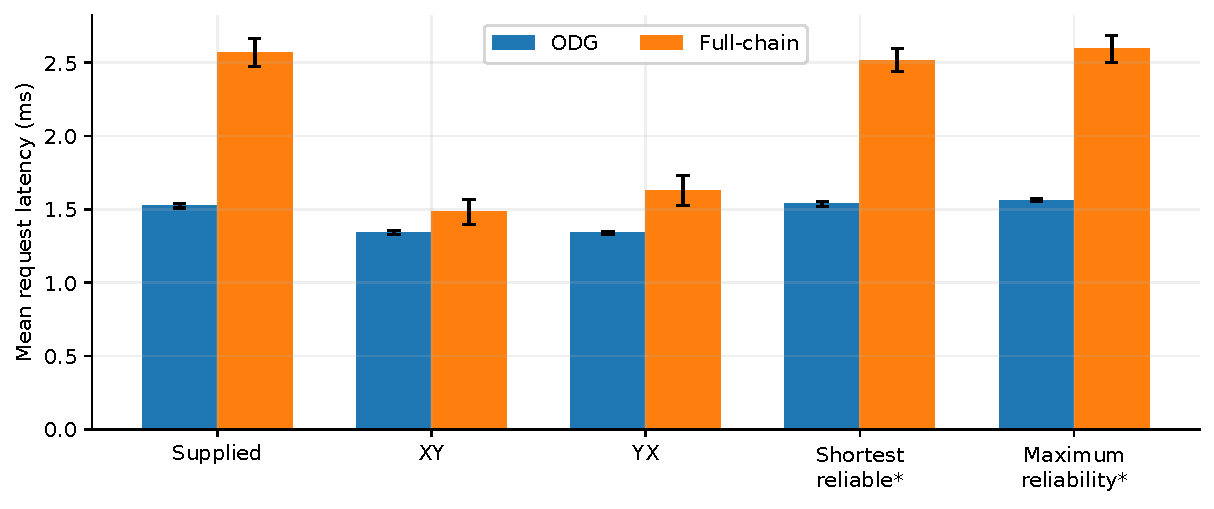
\includegraphics[width=\linewidth,height=0.37\textheight,keepaspectratio]{figures/routing_request_latency_mean_ms.pdf}\captionof{figure}{Mean request latency (ms). Error bars are sample SD across 30 physics seeds; starred routes use a reconstructed reliability map.}\end{center}

\begin{center}\small
\begin{longtable}{lrr}
\caption{Mean request latency (ms); 30 seeds per cell.}\\
\toprule
Route & ODG & Full-chain \\
\midrule\endfirsthead
\toprule
Route & ODG & Full-chain \\
\midrule\endhead
Supplied & $1.526 \pm 0.016$ & $2.570 \pm 0.096$ \\
XY & $1.340 \pm 0.013$ & $1.484 \pm 0.086$ \\
YX & $1.340 \pm 0.012$ & $1.628 \pm 0.101$ \\
Shortest reliable & $1.538 \pm 0.016$ & $2.518 \pm 0.080$ \\
Max reliability & $1.564 \pm 0.012$ & $2.597 \pm 0.092$ \\
\bottomrule\end{longtable}\end{center}
{\footnotesize \href{https://github.com/sanjeevkrishnaa/Compiler-Driven-ACE/blob/codex/ace-scheduler-correctness/docs/latex/oct25_pre_golden/data/routing.csv}{Complete CSV: routing}. }

\clearpage
\begin{center}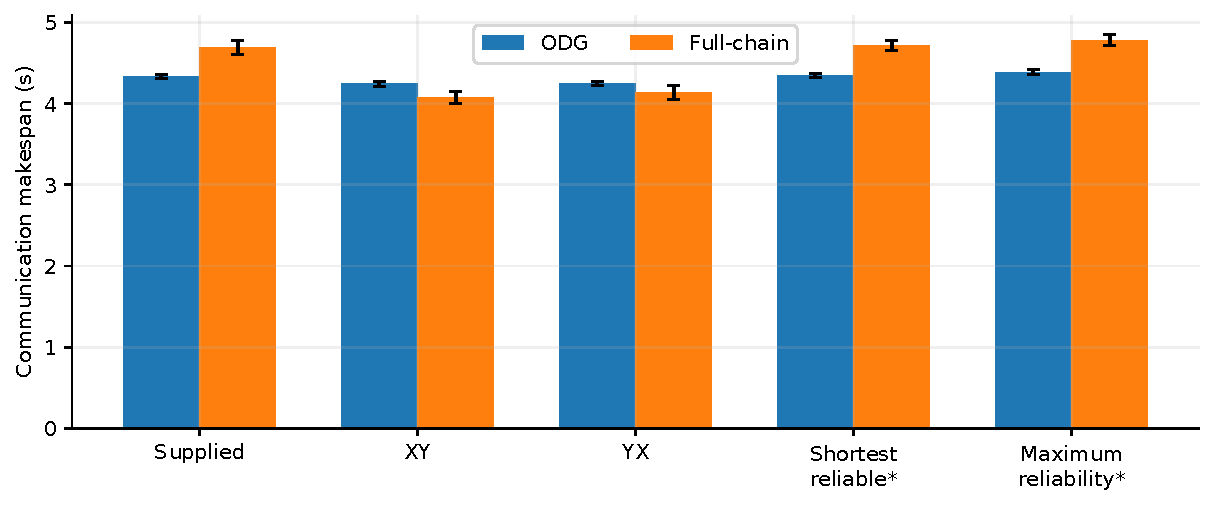
\includegraphics[width=\linewidth,height=0.37\textheight,keepaspectratio]{figures/routing_end_to_end_latency_ms.pdf}\captionof{figure}{Communication makespan (s). Error bars are sample SD across 30 physics seeds; starred routes use a reconstructed reliability map.}\end{center}

\begin{center}\small
\begin{longtable}{lrr}
\caption{Communication makespan (s); 30 seeds per cell.}\\
\toprule
Route & ODG & Full-chain \\
\midrule\endfirsthead
\toprule
Route & ODG & Full-chain \\
\midrule\endhead
Supplied & $4.337 \pm 0.026$ & $4.694 \pm 0.086$ \\
XY & $4.244 \pm 0.031$ & $4.076 \pm 0.070$ \\
YX & $4.247 \pm 0.026$ & $4.136 \pm 0.082$ \\
Shortest reliable & $4.345 \pm 0.024$ & $4.716 \pm 0.061$ \\
Max reliability & $4.387 \pm 0.029$ & $4.781 \pm 0.066$ \\
\bottomrule\end{longtable}\end{center}
{\footnotesize \href{https://github.com/sanjeevkrishnaa/Compiler-Driven-ACE/blob/codex/ace-scheduler-correctness/docs/latex/oct25_pre_golden/data/routing.csv}{Complete CSV: routing}. }

\clearpage
\begin{center}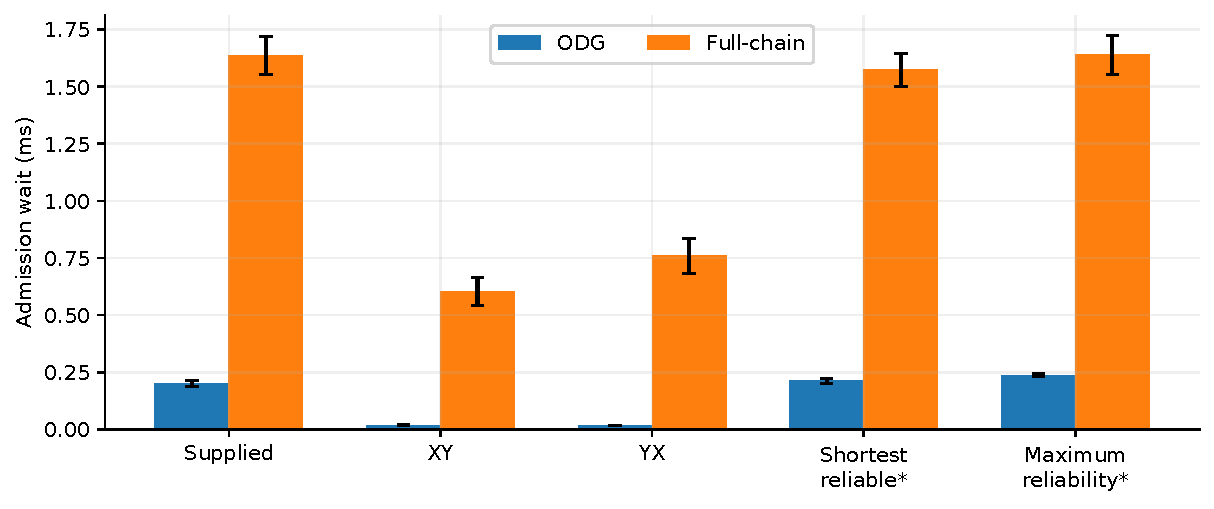
\includegraphics[width=\linewidth,height=0.37\textheight,keepaspectratio]{figures/routing_average_admission_wait_ms.pdf}\captionof{figure}{Admission wait (ms). Error bars are sample SD across 30 physics seeds; starred routes use a reconstructed reliability map.}\end{center}

\begin{center}\small
\begin{longtable}{lrr}
\caption{Admission wait (ms); 30 seeds per cell.}\\
\toprule
Route & ODG & Full-chain \\
\midrule\endfirsthead
\toprule
Route & ODG & Full-chain \\
\midrule\endhead
Supplied & $0.200 \pm 0.012$ & $1.638 \pm 0.083$ \\
XY & $0.018 \pm 0.002$ & $0.603 \pm 0.062$ \\
YX & $0.017 \pm 0.002$ & $0.759 \pm 0.077$ \\
Shortest reliable & $0.212 \pm 0.009$ & $1.574 \pm 0.073$ \\
Max reliability & $0.238 \pm 0.007$ & $1.640 \pm 0.086$ \\
\bottomrule\end{longtable}\end{center}
{\footnotesize \href{https://github.com/sanjeevkrishnaa/Compiler-Driven-ACE/blob/codex/ace-scheduler-correctness/docs/latex/oct25_pre_golden/data/routing.csv}{Complete CSV: routing}. }


\section{Interpretation}
XY and YX reduce Dynamic admission wait and whole-trace makespan relative to supplied routing. With XY, full-chain Dynamic's makespan improves to about 4.076 s against ODG's 4.244 s, even while its mean hop latency remains higher. This is a concrete example of latency and makespan ranking policies differently. The reliability-aware arms do not establish a comparable improvement under the prewritten wait/gap/makespan decision rule.

\chapter{Testing the congestion explanation}
\section{A static proxy, with an explicit definition}
For layer $\ell$ and core $c$, define hop-touch demand
\[
 D_{\ell c}=E_{\ell c}+2R_{\ell c},\qquad
 X_M=\sum_{\ell,c}\max(0,D_{\ell c}-M).
\]
$E$ counts source/destination appearances in migration paths; $R$ counts relay visits. A relay is counted twice because one adjacent hop arrives and another leaves. $X_M$ measures excess static demand. It is \emph{not} a measured simultaneous occupancy, a queued-time total or a proof that these touches must all reserve memory at once. The sequential same-qubit hops and actual booking durations matter in the simulator.

There are also two distinct useful counters: overloaded core-layers count how often demand exceeds $M$, while excess sums the amount of exceedance. XY has lower excess but can have \emph{more} overloaded core-layers than supplied routing. The result supports less concentrated severe overload, not improvement in every possible congestion statistic.

\section{The intervention design}
Sixteen further arms keep every migration's qubit, layer, endpoints and minimum hop count fixed. They mix supplied routing with XY, choose random shortest paths, choose XY/YX with a seeded coin (O1TURN-style), greedily concentrate or balance per-layer load, or reroute migrations touching the hottest one, two or three relay cores. Each arm is evaluated with 30 physics seeds for ODG and full-chain Dynamic.

The \texttt{balance} policy is a greedy rule in migration order, not a proof of a global optimum. The \texttt{concentrate} policy intentionally maximises a local load objective. The seeded XY/YX choice is an offline routing analogue; the experiment does not claim to implement every detail of a hardware O1TURN router.

\begin{center}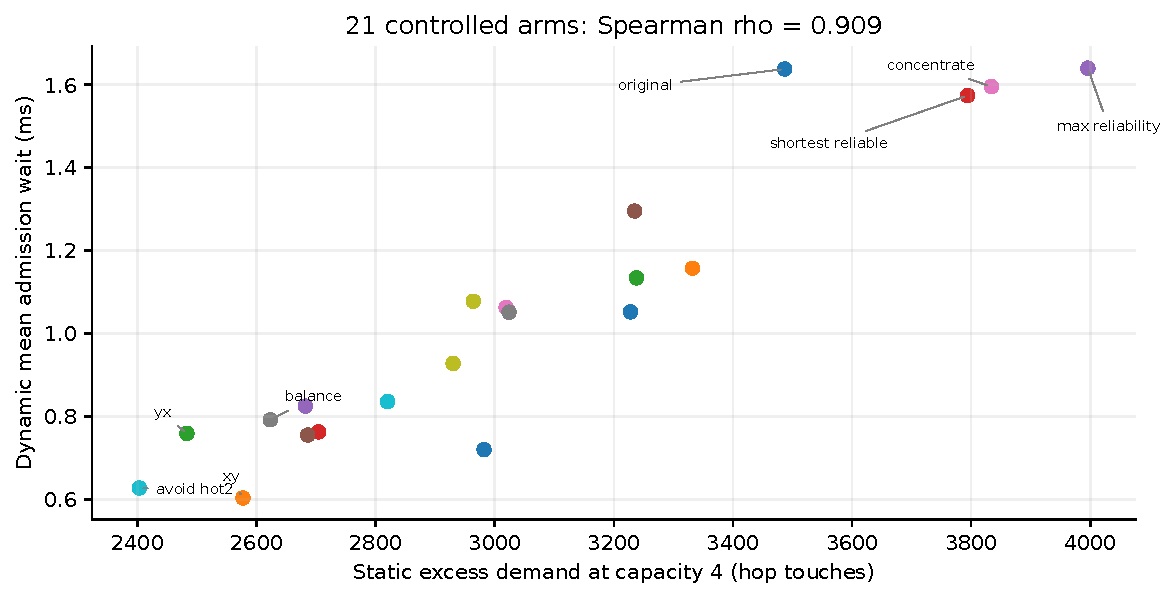
\includegraphics[width=\linewidth,height=0.37\textheight,keepaspectratio]{figures/mechanism.pdf}\captionof{figure}{Static layer demand predicts simulated waiting. Arms are controlled route alternatives sharing endpoints, not 21 independent workload samples.}\end{center}

\begin{center}\small
\begin{longtable}{lrrrr}
\caption{All 21 route alternatives, 30 seeds per policy. Values here are seed means; all SD values are in the unified data CSV.}\\
\toprule
Arm & Excess & ODG ms & Dynamic ms & Wait ms \\
\midrule\endfirsthead
\toprule
Arm & Excess & ODG ms & Dynamic ms & Wait ms \\
\midrule\endhead
original & 3487 & 1.5256 & 2.5701 & 1.6377 \\
xy & 2577 & 1.3401 & 1.4840 & 0.6034 \\
yx & 2483 & 1.3395 & 1.6275 & 0.7589 \\
shortest\_reliable & 3794 & 1.5377 & 2.5181 & 1.5736 \\
max\_reliability & 3996 & 1.5639 & 2.5966 & 1.6398 \\
mix\_p25\_s1 & 3235 & 1.4463 & 2.2112 & 1.2952 \\
mix\_p50\_s1 & 3019 & 1.3953 & 1.9666 & 1.0625 \\
mix\_p50\_s2 & 3024 & 1.3997 & 1.9519 & 1.0513 \\
mix\_p50\_s3 & 2964 & 1.4006 & 1.9826 & 1.0776 \\
mix\_p75\_s1 & 2820 & 1.3669 & 1.7241 & 0.8357 \\
rand\_shortest\_s1 & 3228 & 1.4062 & 1.9764 & 1.0521 \\
rand\_shortest\_s2 & 3332 & 1.4195 & 2.0885 & 1.1573 \\
rand\_shortest\_s3 & 3238 & 1.4194 & 2.0569 & 1.1340 \\
o1turn\_s1 & 2704 & 1.3547 & 1.6494 & 0.7624 \\
o1turn\_s2 & 2682 & 1.3497 & 1.7125 & 0.8248 \\
o1turn\_s3 & 2686 & 1.3489 & 1.6541 & 0.7550 \\
concentrate & 3834 & 1.5849 & 2.5589 & 1.5952 \\
balance & 2623 & 1.3336 & 1.6734 & 0.7918 \\
avoid\_hot1 & 2930 & 1.3999 & 1.8226 & 0.9277 \\
avoid\_hot2 & 2403 & 1.3431 & 1.5030 & 0.6273 \\
avoid\_hot3 & 2982 & 1.3642 & 1.6138 & 0.7196 \\
\bottomrule\end{longtable}\end{center}
{\footnotesize \href{https://github.com/sanjeevkrishnaa/Compiler-Driven-ACE/blob/codex/ace-scheduler-correctness/docs/latex/oct25_pre_golden/data/routing_mechanism.csv}{Complete CSV: routing\_mechanism}. }


The association between excess demand and Dynamic waiting is strong, and deliberate route changes support the load-balancing explanation. However, these 21 arms share a workload and placement and are not independent circuit samples. The concentrate arm has greater excess but its Dynamic/ODG latency \emph{ratio} does not exceed the original ratio: ODG also slows down. This failed part of the original prediction is retained. Ratios alone cannot establish the mechanism.

\section{Where waiting occurs}
\begin{center}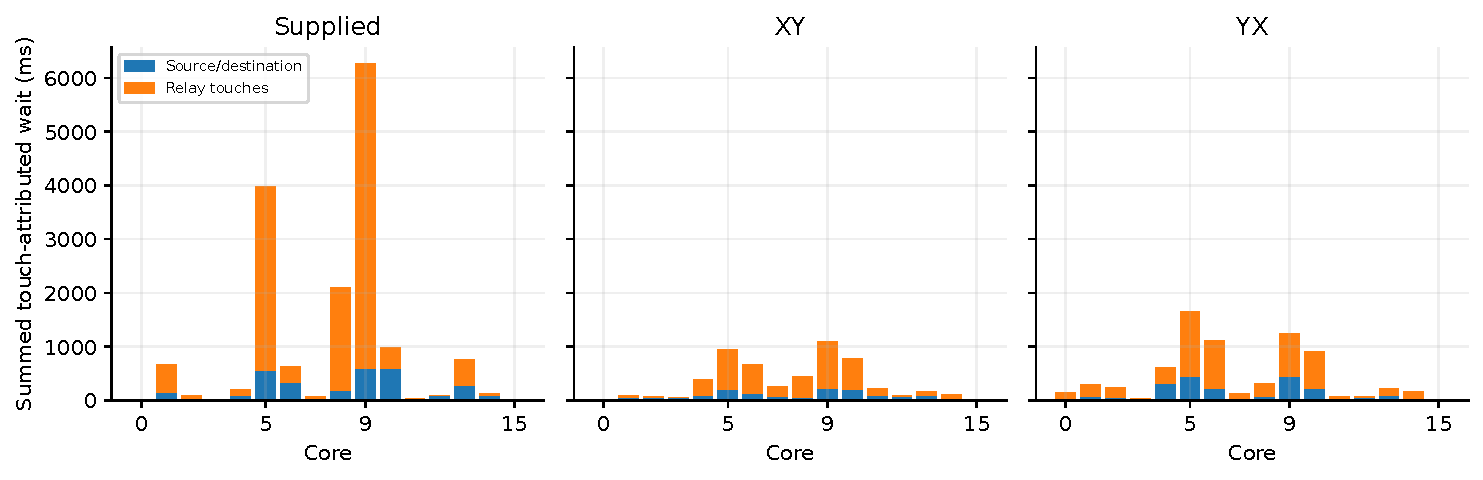
\includegraphics[width=\linewidth,height=0.37\textheight,keepaspectratio]{figures/percore.pdf}\captionof{figure}{Dynamic waiting attributed to endpoint and relay touches, averaged over five physics seeds. A hop touches two cores, so these sums are not wall-clock latency and can count one request twice.}\end{center}

\begin{center}\small
\begin{longtable}{lrrr}
\caption{Complete core-wise values underlying the figure, in ms.}\\
\toprule
Core & Supplied end/relay & XY end/relay & YX end/relay \\
\midrule\endfirsthead
\toprule
Core & Supplied end/relay & XY end/relay & YX end/relay \\
\midrule\endhead
0 & 20.2 / 0.0 & 12.2 / 11.0 & 36.0 / 102.2 \\
1 & 139.4 / 523.6 & 61.3 / 30.2 & 75.0 / 229.5 \\
2 & 36.9 / 63.8 & 49.2 / 24.3 & 51.2 / 197.2 \\
3 & 6.2 / 0.0 & 54.5 / 4.4 & 21.2 / 17.4 \\
4 & 99.3 / 112.9 & 91.5 / 289.2 & 320.5 / 290.7 \\
5 & 561.0 / 3420.2 & 194.3 / 744.6 & 440.4 / 1206.1 \\
6 & 338.0 / 301.4 & 128.8 / 543.7 & 221.9 / 889.5 \\
7 & 40.2 / 36.2 & 69.2 / 198.4 & 41.9 / 82.4 \\
8 & 193.7 / 1912.4 & 53.1 / 397.7 & 78.0 / 240.3 \\
9 & 585.5 / 5675.4 & 222.5 / 867.5 & 436.6 / 800.9 \\
10 & 587.7 / 396.8 & 202.1 / 568.6 & 215.4 / 690.6 \\
11 & 32.7 / 11.0 & 85.3 / 141.4 & 44.7 / 32.0 \\
12 & 90.0 / 0.0 & 69.7 / 26.1 & 60.0 / 10.4 \\
13 & 283.5 / 484.0 & 98.9 / 74.8 & 99.1 / 125.6 \\
14 & 82.7 / 47.9 & 31.8 / 76.7 & 30.0 / 141.2 \\
15 & 4.8 / 4.6 & 9.1 / 17.3 & 5.9 / 9.0 \\
\bottomrule\end{longtable}\end{center}
{\footnotesize \href{https://github.com/sanjeevkrishnaa/Compiler-Driven-ACE/blob/codex/ace-scheduler-correctness/docs/latex/oct25_pre_golden/data/per_core_wait.csv}{Complete CSV: per\_core\_wait}. }

The supplied route's wait is strongly concentrated in a few cores, particularly 5 and 9. Rerouting around two hotspots captures much of the improvement. Endpoint and relay values here are attribution by hop touch; they are not mutually exclusive causal contributions to elapsed time. The same hop's waiting can be attributed to both touched cores.

The original occupancy diagnostic had a documented strategy-label defect when multiple strategies were invoked together. This report therefore uses the correctly identified per-core JSON diagnostics and does not derive numerical occupancy conclusions from those mislabeled files. A source-based explanation is stronger than reusing an attractive but ambiguous plot.

\chapter{Dynamic preparation rules and the launch-policy screen}
\section{What each rule changes}
The Dynamic planner selects candidate preparations subject to memory and generation constraints. Runtime controls change when those preparations launch or filter the set of prepared hops. They do not change the placement or route.

\begin{longtable}{p{.31\linewidth}p{.61\linewidth}}
\toprule Rule & Implemented meaning\\\midrule\endhead
Layer-start & Launch on activation of the planned generation layer. The baseline planner commonly chooses the preceding layer; do not assume every request is always planned exactly one layer early.\\
Preparation delay & Add the chosen delay after the layer trigger for layer-start launches. This differs from the obsolete fixed 5.3 ms lead before demand reservations.\\
Predecessor-start & Register a later-hop preparation to launch when its predecessor hop starts. First hops use the generation-layer rule. A shorter storage interval can come at the cost of the pair being unready.\\
Chain depth $N$ & Keep only preparations for the first $N$ hop positions of each $(\ell,q)$ chain. Other hops remain requests served through fallback. $N=1$ is first-hop-only, not one hop per core or one hop per layer.\\
Combined rules & Chain filtering and trigger changes can be applied together; the 13 named screen variants include delay combinations and two-hop predecessor-start.\\
\bottomrule
\end{longtable}

\section{Ten-seed screening on supplied and XY routes}
All 13 variants are included for each route. The dashed ODG line uses the existing 30-seed reference; therefore the graph is a screen, not a matched-size confirmation. The subsequent confirmation uses 30 seeds for the selected first-hop and adaptive policies too.
\clearpage\subsection{Supplied route}
\begin{center}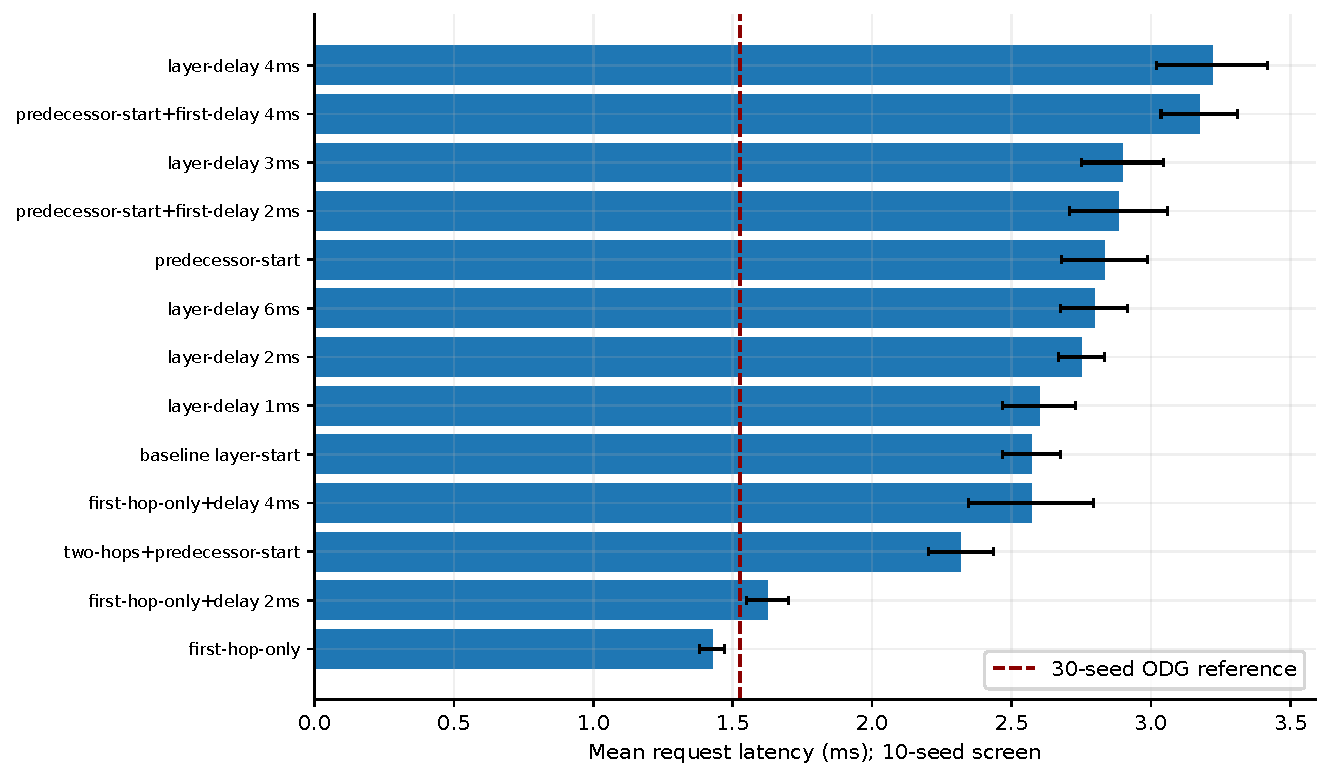
\includegraphics[width=\linewidth,height=0.44\textheight,keepaspectratio]{figures/launch_original.pdf}\captionof{figure}{Every launch-policy screen, including unsuccessful delays and predecessor triggers.}\end{center}

\begin{center}\small
\begin{longtable}{lrrr}
\caption{Timing results; mean $\pm$ SD, 10 seeds.}\\
\toprule
Variant & Latency ms & p95 ms & Makespan s \\
\midrule\endfirsthead
\toprule
Variant & Latency ms & p95 ms & Makespan s \\
\midrule\endhead
first-hop-only & $1.426 \pm 0.043$ & $3.610 \pm 0.202$ & $4.224 \pm 0.023$ \\
first-hop-only+delay 2ms & $1.625 \pm 0.075$ & $4.020 \pm 0.239$ & $4.378 \pm 0.064$ \\
two-hops+predecessor-start & $2.318 \pm 0.116$ & $6.300 \pm 0.634$ & $4.843 \pm 0.098$ \\
first-hop-only+delay 4ms & $2.571 \pm 0.224$ & $6.750 \pm 0.984$ & $5.084 \pm 0.158$ \\
baseline layer-start & $2.573 \pm 0.103$ & $8.480 \pm 0.579$ & $4.709 \pm 0.086$ \\
layer-delay 1ms & $2.599 \pm 0.132$ & $8.520 \pm 0.649$ & $4.728 \pm 0.095$ \\
layer-delay 2ms & $2.751 \pm 0.083$ & $8.710 \pm 0.423$ & $4.848 \pm 0.052$ \\
layer-delay 6ms & $2.796 \pm 0.120$ & $8.820 \pm 0.418$ & $5.091 \pm 0.089$ \\
predecessor-start & $2.833 \pm 0.155$ & $7.760 \pm 0.844$ & $5.196 \pm 0.089$ \\
predecessor-start+first-delay 2ms & $2.884 \pm 0.176$ & $7.790 \pm 0.706$ & $5.252 \pm 0.114$ \\
layer-delay 3ms & $2.899 \pm 0.147$ & $8.840 \pm 0.793$ & $5.008 \pm 0.105$ \\
predecessor-start+first-delay 4ms & $3.173 \pm 0.137$ & $8.420 \pm 0.651$ & $5.448 \pm 0.077$ \\
layer-delay 4ms & $3.219 \pm 0.199$ & $9.690 \pm 0.894$ & $5.243 \pm 0.118$ \\
\bottomrule\end{longtable}\end{center}
{\footnotesize \href{https://github.com/sanjeevkrishnaa/Compiler-Driven-ACE/blob/codex/ace-scheduler-correctness/docs/latex/oct25_pre_golden/data/launch_screen.csv}{Complete CSV: launch\_screen}. }

\clearpage
\begin{center}\small
\begin{longtable}{lrrr}
\caption{Readiness, compiler waste and delivered fidelity for the same screen.}\\
\toprule
Variant & Ready frac. & Waste \% & Delivered F \\
\midrule\endfirsthead
\toprule
Variant & Ready frac. & Waste \% & Delivered F \\
\midrule\endhead
first-hop-only & $0.193 \pm 0.001$ & $0.467 \pm 0.199$ & $0.9483 \pm 0.0000$ \\
first-hop-only+delay 2ms & $0.154 \pm 0.008$ & $2.958 \pm 0.631$ & $0.9491 \pm 0.0000$ \\
two-hops+predecessor-start & $0.178 \pm 0.013$ & $4.344 \pm 0.583$ & $0.9484 \pm 0.0001$ \\
first-hop-only+delay 4ms & $0.039 \pm 0.004$ & $18.405 \pm 1.829$ & $0.9497 \pm 0.0000$ \\
baseline layer-start & $0.434 \pm 0.016$ & $0.518 \pm 0.127$ & $0.9432 \pm 0.0003$ \\
layer-delay 1ms & $0.412 \pm 0.014$ & $0.746 \pm 0.200$ & $0.9441 \pm 0.0003$ \\
layer-delay 2ms & $0.333 \pm 0.025$ & $1.727 \pm 0.376$ & $0.9454 \pm 0.0003$ \\
layer-delay 6ms & $0.130 \pm 0.008$ & $6.108 \pm 0.741$ & $0.9479 \pm 0.0002$ \\
predecessor-start & $0.154 \pm 0.006$ & $7.732 \pm 0.363$ & $0.9487 \pm 0.0001$ \\
predecessor-start+first-delay 2ms & $0.136 \pm 0.008$ & $8.682 \pm 0.654$ & $0.9490 \pm 0.0001$ \\
layer-delay 3ms & $0.264 \pm 0.021$ & $2.987 \pm 0.496$ & $0.9464 \pm 0.0003$ \\
predecessor-start+first-delay 4ms & $0.076 \pm 0.005$ & $14.604 \pm 0.971$ & $0.9494 \pm 0.0001$ \\
layer-delay 4ms & $0.163 \pm 0.011$ & $6.639 \pm 0.683$ & $0.9474 \pm 0.0003$ \\
\bottomrule\end{longtable}\end{center}
{\footnotesize \href{https://github.com/sanjeevkrishnaa/Compiler-Driven-ACE/blob/codex/ace-scheduler-correctness/docs/latex/oct25_pre_golden/data/launch_screen.csv}{Complete CSV: launch\_screen}. }

\clearpage\subsection{XY route}
\begin{center}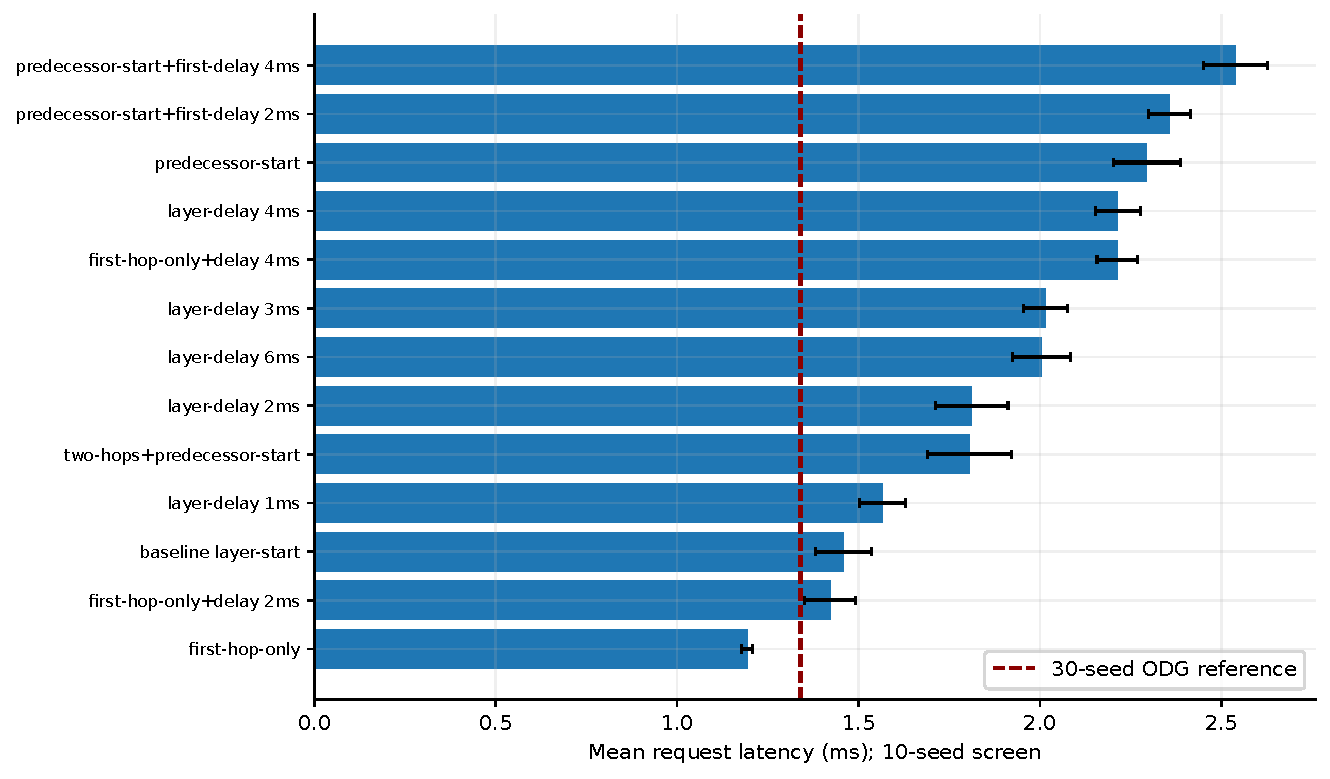
\includegraphics[width=\linewidth,height=0.44\textheight,keepaspectratio]{figures/launch_xy.pdf}\captionof{figure}{Every launch-policy screen, including unsuccessful delays and predecessor triggers.}\end{center}

\begin{center}\small
\begin{longtable}{lrrr}
\caption{Timing results; mean $\pm$ SD, 10 seeds.}\\
\toprule
Variant & Latency ms & p95 ms & Makespan s \\
\midrule\endfirsthead
\toprule
Variant & Latency ms & p95 ms & Makespan s \\
\midrule\endhead
first-hop-only & $1.193 \pm 0.015$ & $2.960 \pm 0.151$ & $4.126 \pm 0.022$ \\
first-hop-only+delay 2ms & $1.422 \pm 0.070$ & $3.560 \pm 0.299$ & $4.311 \pm 0.056$ \\
baseline layer-start & $1.459 \pm 0.077$ & $4.280 \pm 0.278$ & $4.059 \pm 0.070$ \\
layer-delay 1ms & $1.566 \pm 0.063$ & $4.560 \pm 0.222$ & $4.153 \pm 0.050$ \\
two-hops+predecessor-start & $1.806 \pm 0.117$ & $4.800 \pm 0.514$ & $4.536 \pm 0.068$ \\
layer-delay 2ms & $1.812 \pm 0.100$ & $5.190 \pm 0.332$ & $4.341 \pm 0.067$ \\
layer-delay 6ms & $2.004 \pm 0.079$ & $5.600 \pm 0.469$ & $4.596 \pm 0.041$ \\
layer-delay 3ms & $2.016 \pm 0.062$ & $5.530 \pm 0.211$ & $4.511 \pm 0.044$ \\
first-hop-only+delay 4ms & $2.213 \pm 0.055$ & $5.930 \pm 0.211$ & $4.870 \pm 0.055$ \\
layer-delay 4ms & $2.215 \pm 0.062$ & $5.960 \pm 0.288$ & $4.660 \pm 0.054$ \\
predecessor-start & $2.295 \pm 0.092$ & $6.200 \pm 0.350$ & $4.819 \pm 0.058$ \\
predecessor-start+first-delay 2ms & $2.357 \pm 0.058$ & $6.350 \pm 0.255$ & $4.870 \pm 0.035$ \\
predecessor-start+first-delay 4ms & $2.540 \pm 0.088$ & $6.550 \pm 0.295$ & $5.004 \pm 0.051$ \\
\bottomrule\end{longtable}\end{center}
{\footnotesize \href{https://github.com/sanjeevkrishnaa/Compiler-Driven-ACE/blob/codex/ace-scheduler-correctness/docs/latex/oct25_pre_golden/data/launch_screen.csv}{Complete CSV: launch\_screen}. }

\clearpage
\begin{center}\small
\begin{longtable}{lrrr}
\caption{Readiness, compiler waste and delivered fidelity for the same screen.}\\
\toprule
Variant & Ready frac. & Waste \% & Delivered F \\
\midrule\endfirsthead
\toprule
Variant & Ready frac. & Waste \% & Delivered F \\
\midrule\endhead
first-hop-only & $0.226 \pm 0.004$ & $0.469 \pm 0.138$ & $0.9481 \pm 0.0000$ \\
first-hop-only+delay 2ms & $0.169 \pm 0.007$ & $2.726 \pm 0.445$ & $0.9490 \pm 0.0000$ \\
baseline layer-start & $0.506 \pm 0.027$ & $0.456 \pm 0.141$ & $0.9440 \pm 0.0002$ \\
layer-delay 1ms & $0.449 \pm 0.036$ & $0.846 \pm 0.230$ & $0.9453 \pm 0.0003$ \\
two-hops+predecessor-start & $0.182 \pm 0.013$ & $4.129 \pm 0.526$ & $0.9484 \pm 0.0001$ \\
layer-delay 2ms & $0.352 \pm 0.032$ & $1.690 \pm 0.347$ & $0.9467 \pm 0.0002$ \\
layer-delay 6ms & $0.121 \pm 0.007$ & $7.729 \pm 0.571$ & $0.9488 \pm 0.0001$ \\
layer-delay 3ms & $0.266 \pm 0.013$ & $3.136 \pm 0.298$ & $0.9476 \pm 0.0002$ \\
first-hop-only+delay 4ms & $0.037 \pm 0.004$ & $18.740 \pm 1.894$ & $0.9497 \pm 0.0000$ \\
layer-delay 4ms & $0.186 \pm 0.016$ & $5.695 \pm 0.612$ & $0.9481 \pm 0.0002$ \\
predecessor-start & $0.159 \pm 0.015$ & $8.267 \pm 1.027$ & $0.9487 \pm 0.0001$ \\
predecessor-start+first-delay 2ms & $0.140 \pm 0.008$ & $9.348 \pm 0.899$ & $0.9491 \pm 0.0000$ \\
predecessor-start+first-delay 4ms & $0.074 \pm 0.009$ & $15.644 \pm 2.151$ & $0.9495 \pm 0.0001$ \\
\bottomrule\end{longtable}\end{center}
{\footnotesize \href{https://github.com/sanjeevkrishnaa/Compiler-Driven-ACE/blob/codex/ace-scheduler-correctness/docs/latex/oct25_pre_golden/data/launch_screen.csv}{Complete CSV: launch\_screen}. }


\section{What the unsuccessful trials teach}
Simple delay and predecessor-start variants generally reduce readiness and can increase waste or latency. Waiting until a predecessor starts can be too late to avoid generation on the critical path. First-hop-only lowers readiness relative to full-chain but sharply reduces later-hop memory retention, making the remaining cache more useful. A larger hit rate is therefore not by itself an optimisation objective.

\chapter{From first-hop-only to congestion-adaptive preparation}
\section{Thirty-seed confirmation of the selected rules}
The confirmation compares four policies under identical routes: ODG, full-chain Dynamic, first-hop-only Dynamic and threshold-25 Dynamic. Each row compares against ODG on the \emph{same route}. Comparing XY Dynamic only with supplied-route ODG would combine the effects of two interventions.

The adaptive rule computes the target layer's total number of adjacent-hop requests $A_\ell$. It retains a first-hop preparation regardless of $A_\ell$, and retains a later-hop preparation only when $A_\ell\le T$. This is an offline trace-activity proxy, not an online free-memory measurement. Threshold zero equals first-hop-only for layers containing requests; a sufficiently large threshold equals the baseline full-chain rule. The rule filters an existing planner schedule; it does not redistribute freed planner capacity by replanning.

\clearpage\subsection{Mean request latency (ms)}
\begin{center}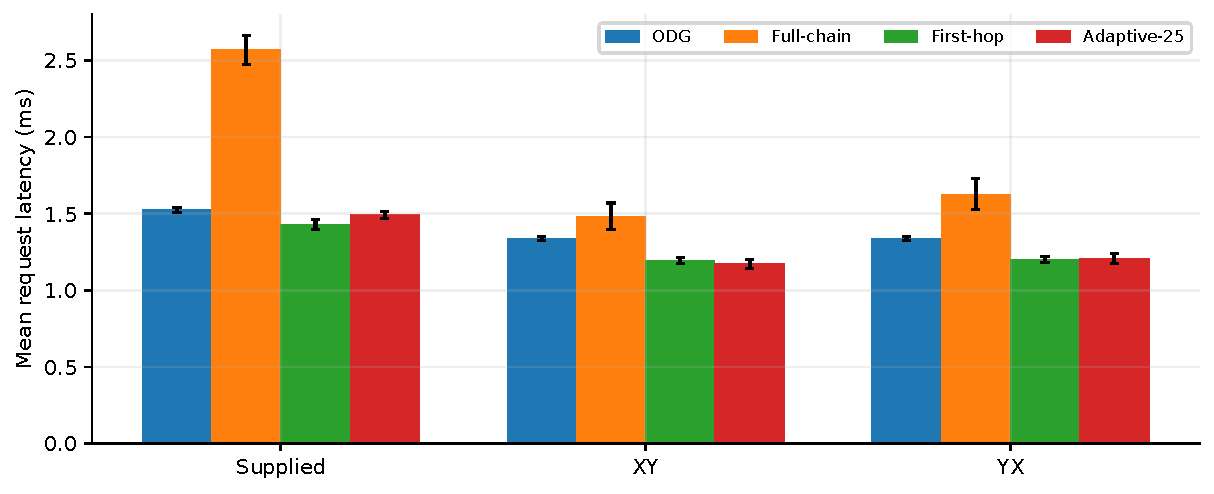
\includegraphics[width=\linewidth,height=0.37\textheight,keepaspectratio]{figures/confirmation_request_latency_mean_ms.pdf}\captionof{figure}{Mean request latency (ms) for the 30-seed confirmation. Error bars show sample SD.}\end{center}

\begin{center}\small
\begin{longtable}{lrrrr}
\caption{Mean request latency (ms); mean $\pm$ SD.}\\
\toprule
Route & ODG & Full-chain & First-hop & Adaptive-25 \\
\midrule\endfirsthead
\toprule
Route & ODG & Full-chain & First-hop & Adaptive-25 \\
\midrule\endhead
Supplied & $1.526 \pm 0.016$ & $2.570 \pm 0.096$ & $1.428 \pm 0.033$ & $1.493 \pm 0.024$ \\
XY & $1.340 \pm 0.013$ & $1.484 \pm 0.086$ & $1.194 \pm 0.018$ & $1.175 \pm 0.029$ \\
YX & $1.340 \pm 0.012$ & $1.628 \pm 0.101$ & $1.200 \pm 0.020$ & $1.207 \pm 0.032$ \\
\bottomrule\end{longtable}\end{center}
{\footnotesize \href{https://github.com/sanjeevkrishnaa/Compiler-Driven-ACE/blob/codex/ace-scheduler-correctness/docs/latex/oct25_pre_golden/data/confirmation.csv}{Complete CSV: confirmation}. }

\clearpage\subsection{Per-run p95 request latency (ms)}
\begin{center}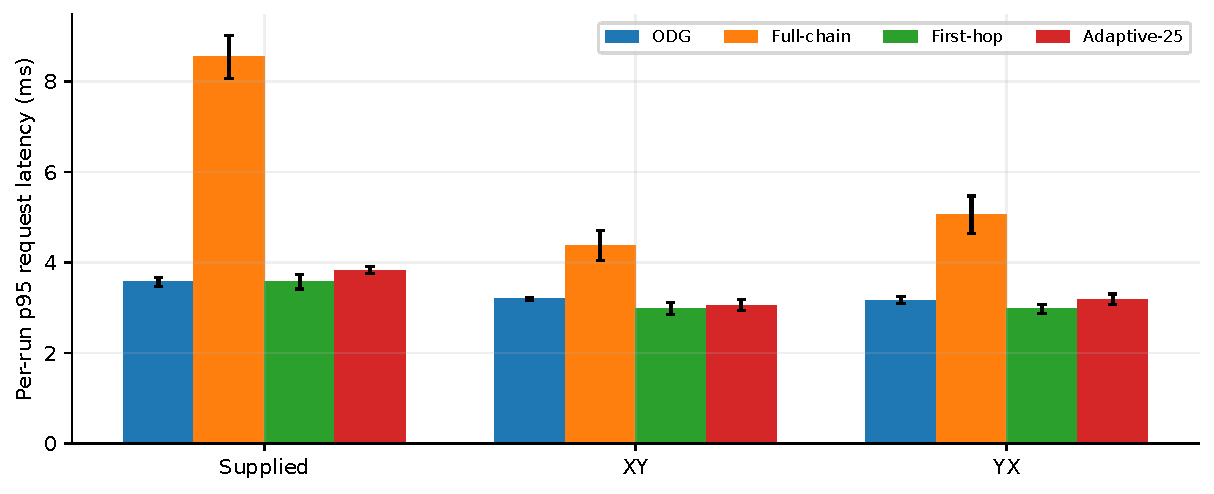
\includegraphics[width=\linewidth,height=0.37\textheight,keepaspectratio]{figures/confirmation_request_latency_p95_ms.pdf}\captionof{figure}{Per-run p95 request latency (ms) for the 30-seed confirmation. Error bars show sample SD.}\end{center}

\begin{center}\small
\begin{longtable}{lrrrr}
\caption{Per-run p95 request latency (ms); mean $\pm$ SD.}\\
\toprule
Route & ODG & Full-chain & First-hop & Adaptive-25 \\
\midrule\endfirsthead
\toprule
Route & ODG & Full-chain & First-hop & Adaptive-25 \\
\midrule\endhead
Supplied & $3.570 \pm 0.099$ & $8.544 \pm 0.478$ & $3.577 \pm 0.163$ & $3.827 \pm 0.078$ \\
XY & $3.193 \pm 0.037$ & $4.373 \pm 0.325$ & $2.977 \pm 0.133$ & $3.060 \pm 0.116$ \\
YX & $3.163 \pm 0.076$ & $5.057 \pm 0.411$ & $2.973 \pm 0.108$ & $3.187 \pm 0.117$ \\
\bottomrule\end{longtable}\end{center}
{\footnotesize \href{https://github.com/sanjeevkrishnaa/Compiler-Driven-ACE/blob/codex/ace-scheduler-correctness/docs/latex/oct25_pre_golden/data/confirmation.csv}{Complete CSV: confirmation}. }

\clearpage\subsection{Communication makespan (s)}
\begin{center}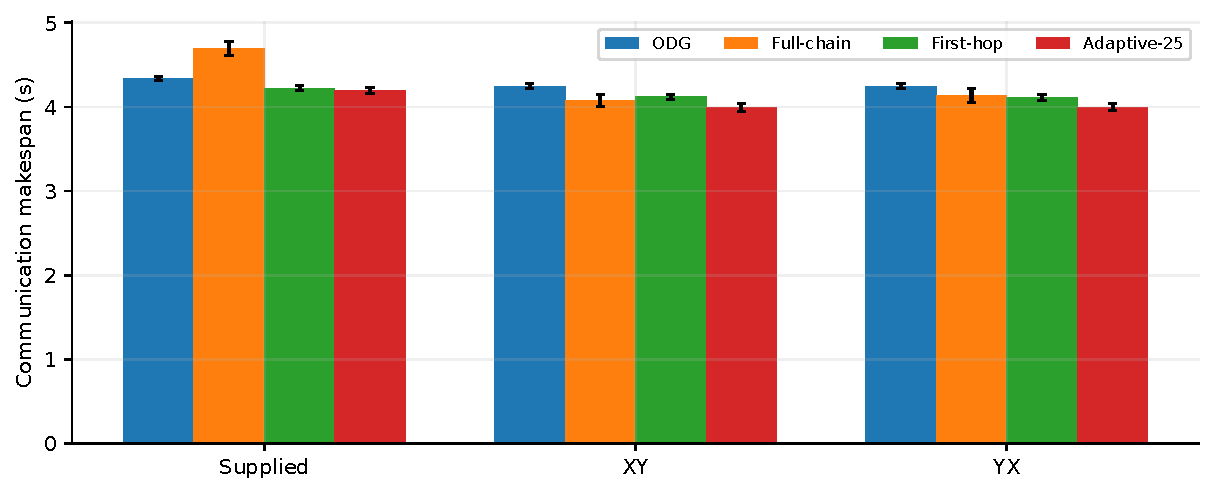
\includegraphics[width=\linewidth,height=0.37\textheight,keepaspectratio]{figures/confirmation_end_to_end_latency_ms.pdf}\captionof{figure}{Communication makespan (s) for the 30-seed confirmation. Error bars show sample SD.}\end{center}

\begin{center}\small
\begin{longtable}{lrrrr}
\caption{Communication makespan (s); mean $\pm$ SD.}\\
\toprule
Route & ODG & Full-chain & First-hop & Adaptive-25 \\
\midrule\endfirsthead
\toprule
Route & ODG & Full-chain & First-hop & Adaptive-25 \\
\midrule\endhead
Supplied & $4.337 \pm 0.026$ & $4.694 \pm 0.086$ & $4.224 \pm 0.025$ & $4.194 \pm 0.034$ \\
XY & $4.244 \pm 0.031$ & $4.076 \pm 0.070$ & $4.120 \pm 0.031$ & $3.992 \pm 0.044$ \\
YX & $4.247 \pm 0.026$ & $4.136 \pm 0.082$ & $4.112 \pm 0.032$ & $3.998 \pm 0.040$ \\
\bottomrule\end{longtable}\end{center}
{\footnotesize \href{https://github.com/sanjeevkrishnaa/Compiler-Driven-ACE/blob/codex/ace-scheduler-correctness/docs/latex/oct25_pre_golden/data/confirmation.csv}{Complete CSV: confirmation}. }

\clearpage\subsection{Admission wait (ms)}
\begin{center}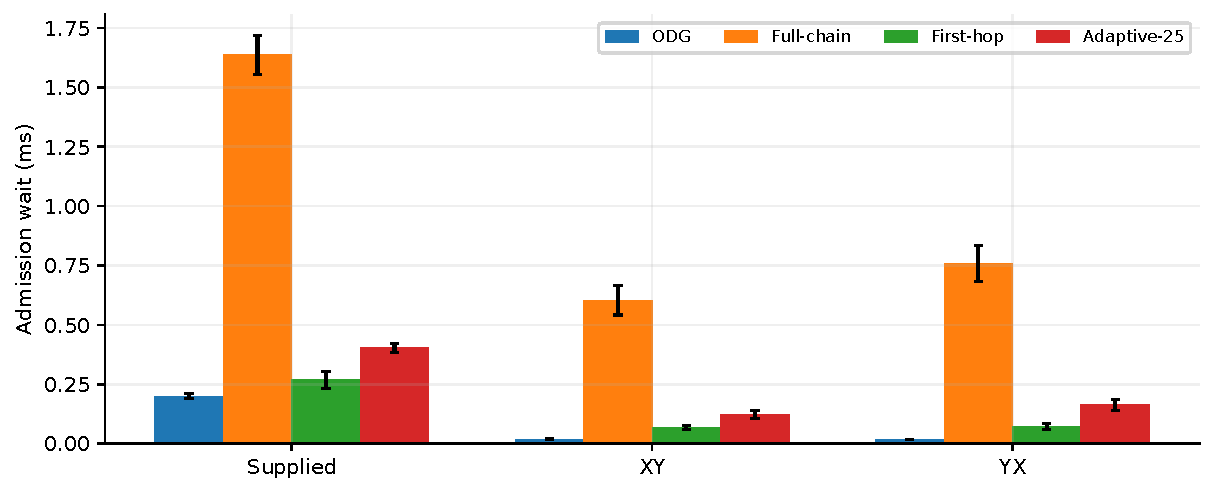
\includegraphics[width=\linewidth,height=0.37\textheight,keepaspectratio]{figures/confirmation_average_admission_wait_ms.pdf}\captionof{figure}{Admission wait (ms) for the 30-seed confirmation. Error bars show sample SD.}\end{center}

\begin{center}\small
\begin{longtable}{lrrrr}
\caption{Admission wait (ms); mean $\pm$ SD.}\\
\toprule
Route & ODG & Full-chain & First-hop & Adaptive-25 \\
\midrule\endfirsthead
\toprule
Route & ODG & Full-chain & First-hop & Adaptive-25 \\
\midrule\endhead
Supplied & $0.200 \pm 0.012$ & $1.638 \pm 0.083$ & $0.268 \pm 0.035$ & $0.403 \pm 0.019$ \\
XY & $0.018 \pm 0.002$ & $0.603 \pm 0.062$ & $0.068 \pm 0.010$ & $0.123 \pm 0.018$ \\
YX & $0.017 \pm 0.002$ & $0.759 \pm 0.077$ & $0.072 \pm 0.013$ & $0.163 \pm 0.024$ \\
\bottomrule\end{longtable}\end{center}
{\footnotesize \href{https://github.com/sanjeevkrishnaa/Compiler-Driven-ACE/blob/codex/ace-scheduler-correctness/docs/latex/oct25_pre_golden/data/confirmation.csv}{Complete CSV: confirmation}. }

\clearpage\subsection{Readiness fraction}
\begin{center}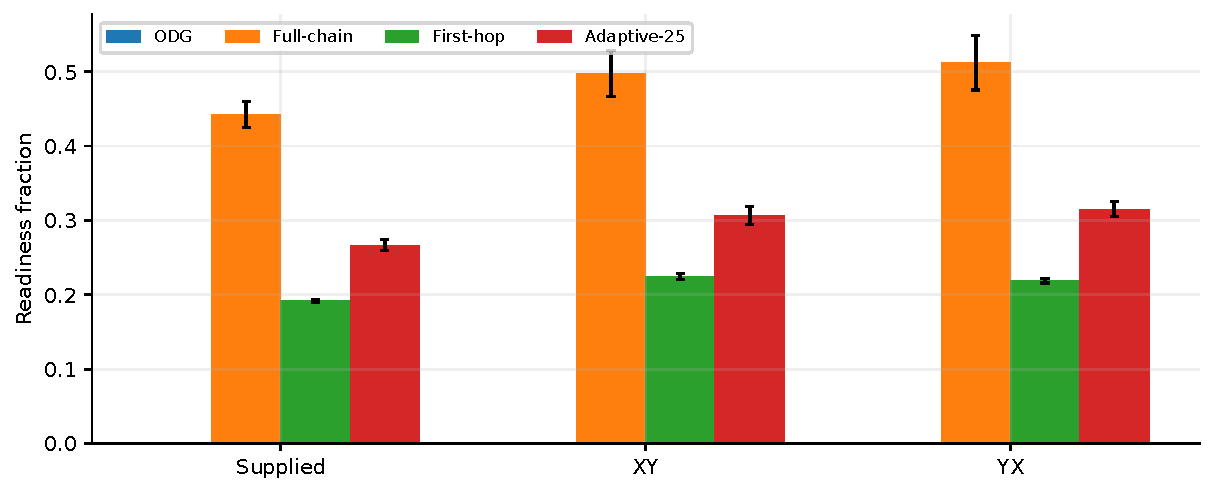
\includegraphics[width=\linewidth,height=0.37\textheight,keepaspectratio]{figures/confirmation_pregenerated_success_rate.pdf}\captionof{figure}{Readiness fraction for the 30-seed confirmation. Error bars show sample SD.}\end{center}

\begin{center}\small
\begin{longtable}{lrrrr}
\caption{Readiness fraction; mean $\pm$ SD.}\\
\toprule
Route & ODG & Full-chain & First-hop & Adaptive-25 \\
\midrule\endfirsthead
\toprule
Route & ODG & Full-chain & First-hop & Adaptive-25 \\
\midrule\endhead
Supplied & $0.000 \pm 0.000$ & $0.443 \pm 0.017$ & $0.192 \pm 0.002$ & $0.266 \pm 0.007$ \\
XY & $0.000 \pm 0.000$ & $0.497 \pm 0.031$ & $0.225 \pm 0.004$ & $0.307 \pm 0.012$ \\
YX & $0.000 \pm 0.000$ & $0.512 \pm 0.037$ & $0.219 \pm 0.003$ & $0.315 \pm 0.010$ \\
\bottomrule\end{longtable}\end{center}
{\footnotesize \href{https://github.com/sanjeevkrishnaa/Compiler-Driven-ACE/blob/codex/ace-scheduler-correctness/docs/latex/oct25_pre_golden/data/confirmation.csv}{Complete CSV: confirmation}. }

\clearpage\subsection{Compiler EPR waste (percent)}
\begin{center}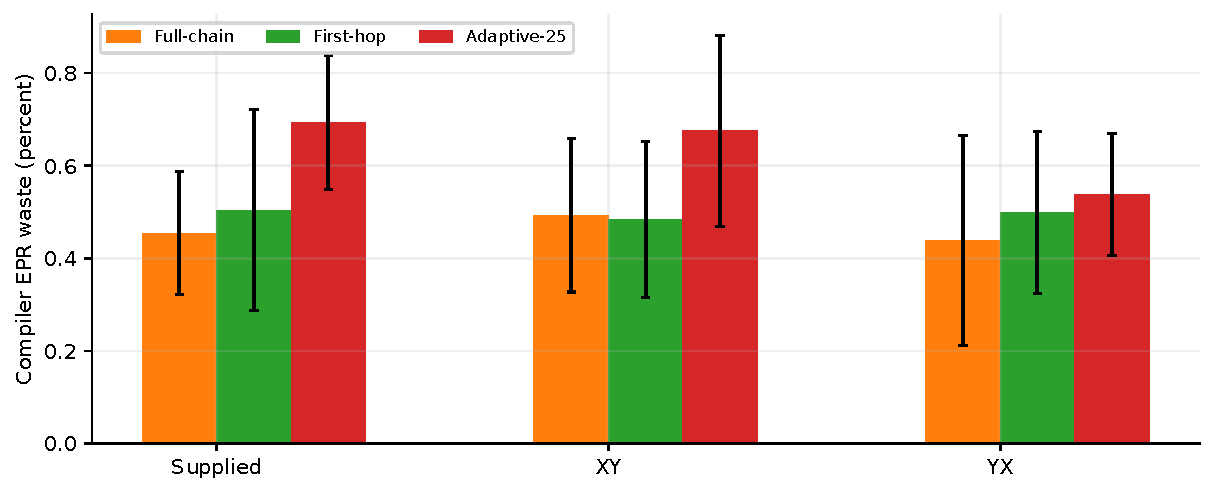
\includegraphics[width=\linewidth,height=0.37\textheight,keepaspectratio]{figures/confirmation_compiler_waste_percentage.pdf}\captionof{figure}{Compiler EPR waste (percent) for the 30-seed confirmation. Error bars show sample SD.}\end{center}

\begin{center}\small
\begin{longtable}{lrrrr}
\caption{Compiler EPR waste (percent); mean $\pm$ SD. ODG has no compiler cache; its zero compiler-waste counter is not an efficiency ratio.}\\
\toprule
Route & ODG & Full-chain & First-hop & Adaptive-25 \\
\midrule\endfirsthead
\toprule
Route & ODG & Full-chain & First-hop & Adaptive-25 \\
\midrule\endhead
Supplied & n/a & $0.454 \pm 0.133$ & $0.504 \pm 0.217$ & $0.693 \pm 0.145$ \\
XY & n/a & $0.493 \pm 0.166$ & $0.483 \pm 0.168$ & $0.675 \pm 0.207$ \\
YX & n/a & $0.438 \pm 0.227$ & $0.499 \pm 0.175$ & $0.539 \pm 0.132$ \\
\bottomrule\end{longtable}\end{center}
{\footnotesize \href{https://github.com/sanjeevkrishnaa/Compiler-Driven-ACE/blob/codex/ace-scheduler-correctness/docs/latex/oct25_pre_golden/data/confirmation.csv}{Complete CSV: confirmation}. }

\clearpage\subsection{Delivered EPR fidelity}
\begin{center}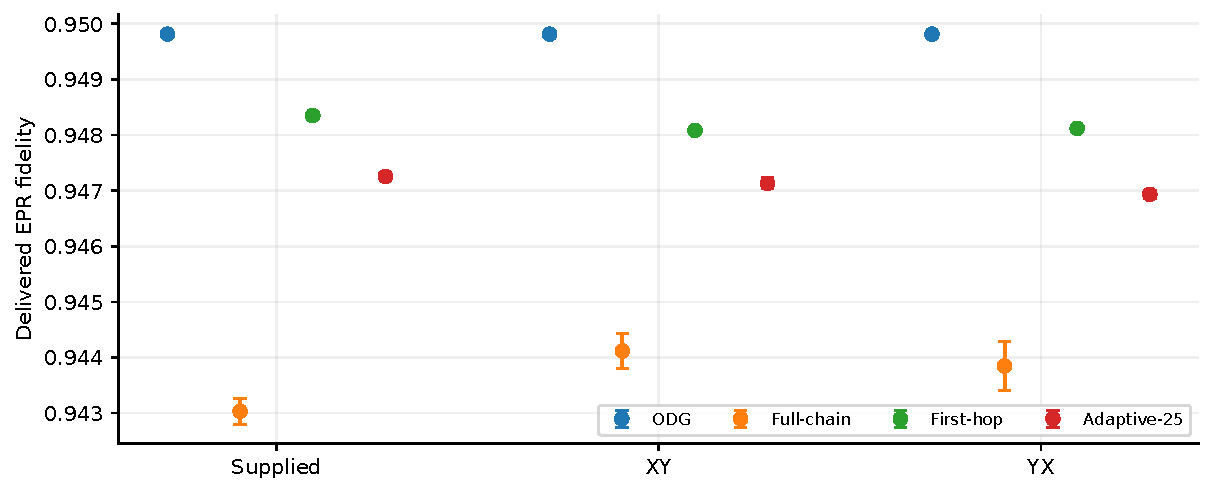
\includegraphics[width=\linewidth,height=0.37\textheight,keepaspectratio]{figures/confirmation_average_delivered_epr_fidelity.pdf}\captionof{figure}{Delivered EPR fidelity for the 30-seed confirmation. Error bars show sample SD.}\end{center}

\begin{center}\small
\begin{longtable}{lrrrr}
\caption{Delivered EPR fidelity; mean $\pm$ SD.}\\
\toprule
Route & ODG & Full-chain & First-hop & Adaptive-25 \\
\midrule\endfirsthead
\toprule
Route & ODG & Full-chain & First-hop & Adaptive-25 \\
\midrule\endhead
Supplied & $0.9498 \pm 0.0000$ & $0.9430 \pm 0.0002$ & $0.9484 \pm 0.0000$ & $0.9473 \pm 0.0001$ \\
XY & $0.9498 \pm 0.0000$ & $0.9441 \pm 0.0003$ & $0.9481 \pm 0.0000$ & $0.9471 \pm 0.0001$ \\
YX & $0.9498 \pm 0.0000$ & $0.9438 \pm 0.0004$ & $0.9481 \pm 0.0000$ & $0.9469 \pm 0.0001$ \\
\bottomrule\end{longtable}\end{center}
{\footnotesize \href{https://github.com/sanjeevkrishnaa/Compiler-Driven-ACE/blob/codex/ace-scheduler-correctness/docs/latex/oct25_pre_golden/data/confirmation.csv}{Complete CSV: confirmation}. }

\clearpage\subsection{Used compiler-pair storage (ms)}
\begin{center}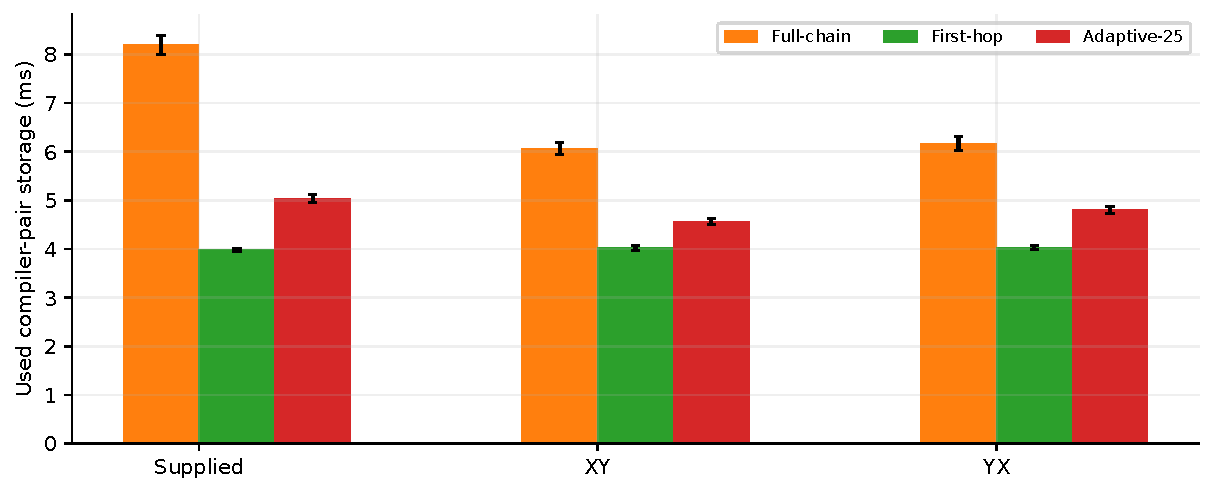
\includegraphics[width=\linewidth,height=0.37\textheight,keepaspectratio]{figures/confirmation_average_storage_time_ms.pdf}\captionof{figure}{Used compiler-pair storage (ms) for the 30-seed confirmation. Error bars show sample SD.}\end{center}

\begin{center}\small
\begin{longtable}{lrrrr}
\caption{Used compiler-pair storage (ms); mean $\pm$ SD.}\\
\toprule
Route & ODG & Full-chain & First-hop & Adaptive-25 \\
\midrule\endfirsthead
\toprule
Route & ODG & Full-chain & First-hop & Adaptive-25 \\
\midrule\endhead
Supplied & n/a & $8.204 \pm 0.196$ & $3.981 \pm 0.037$ & $5.036 \pm 0.082$ \\
XY & n/a & $6.061 \pm 0.122$ & $4.022 \pm 0.045$ & $4.571 \pm 0.063$ \\
YX & n/a & $6.167 \pm 0.150$ & $4.037 \pm 0.043$ & $4.803 \pm 0.074$ \\
\bottomrule\end{longtable}\end{center}
{\footnotesize \href{https://github.com/sanjeevkrishnaa/Compiler-Driven-ACE/blob/codex/ace-scheduler-correctness/docs/latex/oct25_pre_golden/data/confirmation.csv}{Complete CSV: confirmation}. }


\section{What the comparisons establish}
On XY, threshold-25 Dynamic improves mean latency relative to the same-route ODG baseline and has a shorter makespan. First-hop-only also improves both. On supplied routing, first-hop-only gives a lower mean latency than threshold 25. On YX, the two are close, with first-hop-only slightly better in mean latency. A single absolute threshold is therefore not the best preparation rule for every route.

Pre-generation's fidelity remains below ODG's fresh-pair fidelity in the principal comparison. The reduced latency is a measured benefit under the chosen fidelity acceptance and coherence settings; it is not a claim of simultaneous improvement in every metric. Compiler-waste percentages depend on the workload-stop accounting horizon and cannot be interpreted as total system energy waste.

\section{How the threshold was selected}
\begin{center}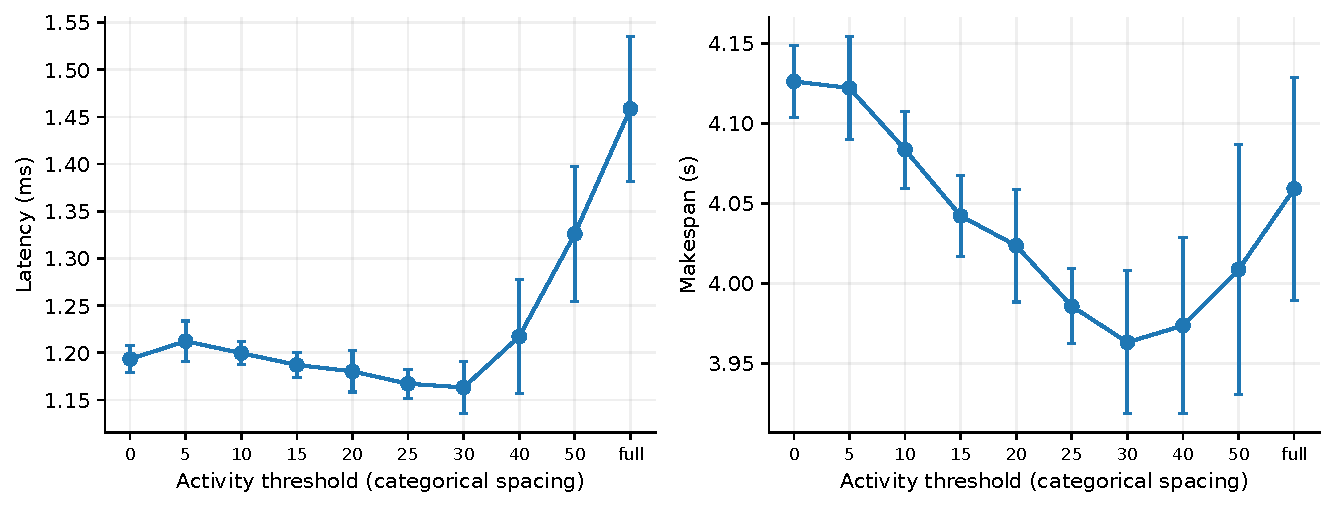
\includegraphics[width=\linewidth,height=0.37\textheight,keepaspectratio]{figures/threshold.pdf}\captionof{figure}{Ten-seed threshold screen on XY. Zero is first-hop-only; the large sentinel is full-chain. The threshold was selected on this same workload.}\end{center}

\begin{center}\small
\begin{longtable}{lrrr}
\caption{Complete threshold screen, 10 seeds per point.}\\
\toprule
Threshold & Latency ms & p95 ms & Makespan s \\
\midrule\endfirsthead
\toprule
Threshold & Latency ms & p95 ms & Makespan s \\
\midrule\endhead
0 & $1.193 \pm 0.015$ & $2.960 \pm 0.151$ & $4.126 \pm 0.022$ \\
5 & $1.212 \pm 0.021$ & $3.080 \pm 0.092$ & $4.122 \pm 0.032$ \\
10 & $1.200 \pm 0.012$ & $3.050 \pm 0.097$ & $4.084 \pm 0.024$ \\
15 & $1.187 \pm 0.014$ & $3.020 \pm 0.079$ & $4.042 \pm 0.026$ \\
20 & $1.180 \pm 0.022$ & $3.010 \pm 0.120$ & $4.024 \pm 0.035$ \\
25 & $1.167 \pm 0.016$ & $3.080 \pm 0.092$ & $3.986 \pm 0.024$ \\
30 & $1.163 \pm 0.028$ & $3.050 \pm 0.127$ & $3.963 \pm 0.045$ \\
40 & $1.217 \pm 0.061$ & $3.290 \pm 0.185$ & $3.974 \pm 0.055$ \\
50 & $1.326 \pm 0.072$ & $3.780 \pm 0.244$ & $4.009 \pm 0.078$ \\
Full & $1.459 \pm 0.077$ & $4.280 \pm 0.278$ & $4.059 \pm 0.070$ \\
\bottomrule\end{longtable}\end{center}
{\footnotesize \href{https://github.com/sanjeevkrishnaa/Compiler-Driven-ACE/blob/codex/ace-scheduler-correctness/docs/latex/oct25_pre_golden/data/threshold.csv}{Complete CSV: threshold}. }

The 10-seed XY screen suggests the region around 25--30. The later 30-seed runs test threshold 25 on three routes. They do not prove an optimal threshold, independence from workload size, or robustness to a changed physical coherence model. Thresholds 25 and 30 are empirically selected settings, not physical constants. A scale-aware or per-core predictor is future research, not a result of this study.

\chapter{Memory allocation and admission screens}
\begin{center}\small
\begin{longtable}{lrrrr}
\caption{All 11 XY first-hop parameter screens, 10 seeds per point. Polling wait is not comparable.}\\
\toprule
Point & M/C & Latency ms & Wait ms & Makespan s \\
\midrule\endfirsthead
\toprule
Point & M/C & Latency ms & Wait ms & Makespan s \\
\midrule\endhead
admission\_poll & 4/3 & $1.459 \pm 0.326$ & n/a & $4.515 \pm 0.532$ \\
cm1\_tm4 & 4/1 & $1.267 \pm 0.014$ & $0.021 \pm 0.002$ & $4.187 \pm 0.030$ \\
cm1\_tm6 & 6/1 & $1.248 \pm 0.011$ & $0.000 \pm 0.000$ & $4.187 \pm 0.024$ \\
cm1\_tm8 & 8/1 & $1.247 \pm 0.011$ & $0.000 \pm 0.000$ & $4.186 \pm 0.025$ \\
cm2\_tm4 & 4/2 & $1.215 \pm 0.014$ & $0.033 \pm 0.003$ & $4.153 \pm 0.020$ \\
cm2\_tm6 & 6/2 & $1.181 \pm 0.013$ & $0.000 \pm 0.000$ & $4.135 \pm 0.014$ \\
cm2\_tm8 & 8/2 & $1.181 \pm 0.013$ & $0.000 \pm 0.000$ & $4.136 \pm 0.014$ \\
cm3\_tm4 & 4/3 & $1.193 \pm 0.015$ & $0.066 \pm 0.007$ & $4.126 \pm 0.022$ \\
cm3\_tm6 & 6/3 & $1.133 \pm 0.012$ & $0.001 \pm 0.000$ & $4.089 \pm 0.019$ \\
cm3\_tm8 & 8/3 & $1.132 \pm 0.012$ & $0.000 \pm 0.000$ & $4.088 \pm 0.021$ \\
no\_starvation\_guard & 4/3 & $1.191 \pm 0.016$ & $0.062 \pm 0.007$ & $4.129 \pm 0.024$ \\
\bottomrule\end{longtable}\end{center}
{\footnotesize \href{https://github.com/sanjeevkrishnaa/Compiler-Driven-ACE/blob/codex/ace-scheduler-correctness/docs/latex/oct25_pre_golden/data/parameter_grid.csv}{Complete CSV: parameter\_grid}. }

These runs all use first-hop-only on XY. Increasing the compiler cap from one to three while keeping total memory at four improves this particular policy, whereas the earlier full-chain diagnosis favoured restricting long-lived cache occupancy. The two observations are compatible: the value of cache capacity depends on which preparations are allowed to hold it.

Total memories six and eight are capacity sensitivity cases relative to the four-memory reference. They should not be described as the same physical hardware. Event versus poll admission changes scheduling behaviour, not just an output label. Polling's wait counter is not comparable; its zero is shown as n/a here. Removing the starvation guard has little effect in this screen, but that is not evidence that starvation protection is unnecessary for every trace and policy.

\chapter{Generalisation to ten archived workloads}
These tests use the archived 48-qubit corpus produced with HQA and OEE initial placement, mapping/reliability seed 42 and physics seeds 0--2. The QFT in this chapter is QFT-48, not QFT-96. Both supplied and XY routes were run with ODG, full-chain Dynamic and first-hop-only. Thresholds 25 and 30 were tested on XY only. There is no evidence here for an all-route adaptive generalisation matrix or a QPE result.

The charts report ratios of means and the tables preserve absolute latency, makespan, fidelity, readiness and waste. A ratio near one under only three seeds should not be described as a universal win. The per-seed CSV also retains p95, fallback, expiry and storage metrics.
\section{Supplied routing: ten 48-qubit workloads}
\begin{center}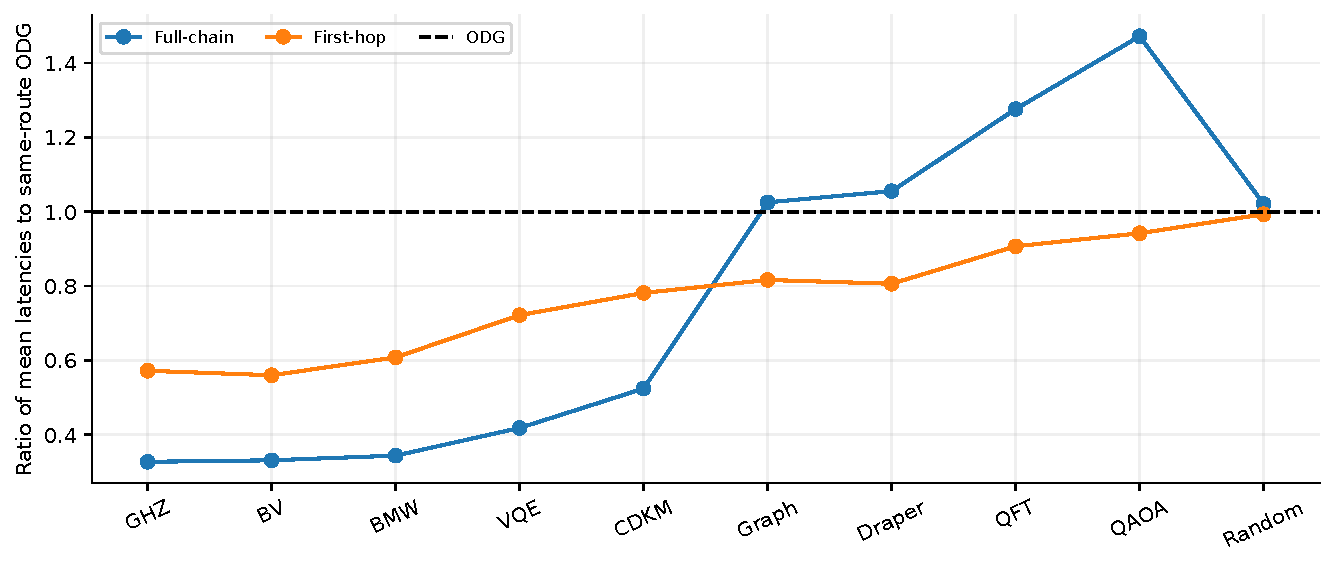
\includegraphics[width=\linewidth,height=0.37\textheight,keepaspectratio]{figures/generalisation_original.pdf}\captionof{figure}{Ratios of seed means, three physics seeds per policy. Workload categories have no continuous order. Ratios have no confidence intervals here.}\end{center}

\begin{center}\small
\begin{longtable}{lrr}
\caption{Exact latency ratios plotted above; values below one favour the listed Dynamic policy.}\\
\toprule
Workload & Full-chain & First-hop \\
\midrule\endfirsthead
\toprule
Workload & Full-chain & First-hop \\
\midrule\endhead
GHZ & 0.3274 & 0.5723 \\
BV & 0.3315 & 0.5602 \\
BMW & 0.3441 & 0.6084 \\
VQE & 0.4184 & 0.7218 \\
CDKM & 0.5244 & 0.7816 \\
Graph & 1.0252 & 0.8165 \\
Draper & 1.0553 & 0.8062 \\
QFT & 1.2759 & 0.9070 \\
QAOA & 1.4718 & 0.9420 \\
Random & 1.0209 & 0.9932 \\
\bottomrule\end{longtable}\end{center}
{\footnotesize \href{https://github.com/sanjeevkrishnaa/Compiler-Driven-ACE/blob/codex/ace-scheduler-correctness/docs/latex/oct25_pre_golden/data/generalisation.csv}{Complete CSV: generalisation}. }

\begin{center}\small
\begin{longtable}{lrrr}
\caption{Latency (ms), mean $\pm$ SD across three seeds.}\\
\toprule
Workload & ODG & Full-chain & First-hop \\
\midrule\endfirsthead
\toprule
Workload & ODG & Full-chain & First-hop \\
\midrule\endhead
GHZ & $1.413 \pm 0.131$ & $0.463 \pm 0.000$ & $0.808 \pm 0.070$ \\
BV & $1.440 \pm 0.142$ & $0.477 \pm 0.058$ & $0.807 \pm 0.054$ \\
BMW & $1.315 \pm 0.055$ & $0.452 \pm 0.004$ & $0.800 \pm 0.016$ \\
VQE & $1.346 \pm 0.046$ & $0.563 \pm 0.023$ & $0.971 \pm 0.051$ \\
CDKM & $1.339 \pm 0.028$ & $0.702 \pm 0.030$ & $1.046 \pm 0.018$ \\
Graph & $1.391 \pm 0.075$ & $1.426 \pm 0.217$ & $1.136 \pm 0.040$ \\
Draper & $1.339 \pm 0.021$ & $1.413 \pm 0.038$ & $1.079 \pm 0.010$ \\
QFT & $1.414 \pm 0.018$ & $1.804 \pm 0.145$ & $1.282 \pm 0.022$ \\
QAOA & $1.362 \pm 0.013$ & $2.005 \pm 0.068$ & $1.283 \pm 0.055$ \\
Random & $1.310 \pm 0.007$ & $1.338 \pm 0.012$ & $1.301 \pm 0.023$ \\
\bottomrule\end{longtable}\end{center}
{\footnotesize \href{https://github.com/sanjeevkrishnaa/Compiler-Driven-ACE/blob/codex/ace-scheduler-correctness/docs/latex/oct25_pre_golden/data/generalisation.csv}{Complete CSV: generalisation}. }

\begin{center}\small
\begin{longtable}{lrrr}
\caption{Makespan (s), mean $\pm$ SD across three seeds.}\\
\toprule
Workload & ODG & Full-chain & First-hop \\
\midrule\endfirsthead
\toprule
Workload & ODG & Full-chain & First-hop \\
\midrule\endhead
GHZ & $0.204 \pm 0.003$ & $0.181 \pm 0.000$ & $0.189 \pm 0.002$ \\
BV & $0.761 \pm 0.004$ & $0.737 \pm 0.001$ & $0.745 \pm 0.001$ \\
BMW & $6.219 \pm 0.008$ & $6.095 \pm 0.001$ & $6.145 \pm 0.002$ \\
VQE & $0.338 \pm 0.006$ & $0.277 \pm 0.001$ & $0.315 \pm 0.004$ \\
CDKM & $3.364 \pm 0.013$ & $3.076 \pm 0.015$ & $3.232 \pm 0.007$ \\
Graph & $0.129 \pm 0.004$ & $0.119 \pm 0.004$ & $0.121 \pm 0.001$ \\
Draper & $2.388 \pm 0.010$ & $2.283 \pm 0.025$ & $2.271 \pm 0.006$ \\
QFT & $2.116 \pm 0.045$ & $2.150 \pm 0.065$ & $2.059 \pm 0.007$ \\
QAOA & $2.082 \pm 0.028$ & $2.347 \pm 0.023$ & $2.003 \pm 0.024$ \\
Random & $14.990 \pm 0.031$ & $14.284 \pm 0.035$ & $14.490 \pm 0.100$ \\
\bottomrule\end{longtable}\end{center}
{\footnotesize \href{https://github.com/sanjeevkrishnaa/Compiler-Driven-ACE/blob/codex/ace-scheduler-correctness/docs/latex/oct25_pre_golden/data/generalisation.csv}{Complete CSV: generalisation}. }

\begin{center}\small
\begin{longtable}{lrrr}
\caption{Delivered fidelity, mean $\pm$ SD across three seeds.}\\
\toprule
Workload & ODG & Full-chain & First-hop \\
\midrule\endfirsthead
\toprule
Workload & ODG & Full-chain & First-hop \\
\midrule\endhead
GHZ & $0.9498 \pm 0.0000$ & $0.9417 \pm 0.0002$ & $0.9451 \pm 0.0002$ \\
BV & $0.9498 \pm 0.0000$ & $0.9416 \pm 0.0002$ & $0.9450 \pm 0.0001$ \\
BMW & $0.9498 \pm 0.0000$ & $0.9415 \pm 0.0001$ & $0.9450 \pm 0.0001$ \\
VQE & $0.9498 \pm 0.0000$ & $0.9422 \pm 0.0001$ & $0.9460 \pm 0.0001$ \\
CDKM & $0.9498 \pm 0.0000$ & $0.9439 \pm 0.0003$ & $0.9474 \pm 0.0000$ \\
Graph & $0.9498 \pm 0.0000$ & $0.9446 \pm 0.0010$ & $0.9485 \pm 0.0002$ \\
Draper & $0.9498 \pm 0.0000$ & $0.9444 \pm 0.0004$ & $0.9469 \pm 0.0001$ \\
QFT & $0.9498 \pm 0.0000$ & $0.9451 \pm 0.0005$ & $0.9481 \pm 0.0000$ \\
QAOA & $0.9498 \pm 0.0000$ & $0.9457 \pm 0.0003$ & $0.9478 \pm 0.0000$ \\
Random & $0.9498 \pm 0.0000$ & $0.9472 \pm 0.0001$ & $0.9483 \pm 0.0000$ \\
\bottomrule\end{longtable}\end{center}
{\footnotesize \href{https://github.com/sanjeevkrishnaa/Compiler-Driven-ACE/blob/codex/ace-scheduler-correctness/docs/latex/oct25_pre_golden/data/generalisation.csv}{Complete CSV: generalisation}. }

\begin{center}\small
\begin{longtable}{lrrr}
\caption{Readiness fraction, mean $\pm$ SD across three seeds.}\\
\toprule
Workload & ODG & Full-chain & First-hop \\
\midrule\endfirsthead
\toprule
Workload & ODG & Full-chain & First-hop \\
\midrule\endhead
GHZ & $0.000 \pm 0.000$ & $1.000 \pm 0.000$ & $0.625 \pm 0.000$ \\
BV & $0.000 \pm 0.000$ & $0.987 \pm 0.023$ & $0.627 \pm 0.023$ \\
BMW & $0.000 \pm 0.000$ & $0.998 \pm 0.004$ & $0.625 \pm 0.000$ \\
VQE & $0.000 \pm 0.000$ & $0.939 \pm 0.015$ & $0.471 \pm 0.000$ \\
CDKM & $0.000 \pm 0.000$ & $0.703 \pm 0.032$ & $0.332 \pm 0.003$ \\
Graph & $0.000 \pm 0.000$ & $0.561 \pm 0.088$ & $0.250 \pm 0.023$ \\
Draper & $0.000 \pm 0.000$ & $0.523 \pm 0.029$ & $0.353 \pm 0.003$ \\
QFT & $0.000 \pm 0.000$ & $0.409 \pm 0.056$ & $0.223 \pm 0.006$ \\
QAOA & $0.000 \pm 0.000$ & $0.350 \pm 0.018$ & $0.252 \pm 0.003$ \\
Random & $0.000 \pm 0.000$ & $0.285 \pm 0.007$ & $0.216 \pm 0.003$ \\
\bottomrule\end{longtable}\end{center}
{\footnotesize \href{https://github.com/sanjeevkrishnaa/Compiler-Driven-ACE/blob/codex/ace-scheduler-correctness/docs/latex/oct25_pre_golden/data/generalisation.csv}{Complete CSV: generalisation}. }

\begin{center}\small
\begin{longtable}{lrrr}
\caption{Compiler waste (percent), mean $\pm$ SD across three seeds.}\\
\toprule
Workload & ODG & Full-chain & First-hop \\
\midrule\endfirsthead
\toprule
Workload & ODG & Full-chain & First-hop \\
\midrule\endhead
GHZ & n/a & $0.000 \pm 0.000$ & $0.000 \pm 0.000$ \\
BV & n/a & $0.000 \pm 0.000$ & $0.000 \pm 0.000$ \\
BMW & n/a & $0.231 \pm 0.401$ & $0.000 \pm 0.000$ \\
VQE & n/a & $0.340 \pm 0.589$ & $0.000 \pm 0.000$ \\
CDKM & n/a & $2.086 \pm 0.837$ & $1.062 \pm 0.368$ \\
Graph & n/a & $4.527 \pm 2.777$ & $6.349 \pm 7.274$ \\
Draper & n/a & $1.157 \pm 0.491$ & $0.216 \pm 0.216$ \\
QFT & n/a & $1.335 \pm 0.446$ & $1.593 \pm 0.563$ \\
QAOA & n/a & $1.239 \pm 0.215$ & $0.509 \pm 0.129$ \\
Random & n/a & $4.187 \pm 0.142$ & $4.819 \pm 0.211$ \\
\bottomrule\end{longtable}\end{center}
{\footnotesize \href{https://github.com/sanjeevkrishnaa/Compiler-Driven-ACE/blob/codex/ace-scheduler-correctness/docs/latex/oct25_pre_golden/data/generalisation.csv}{Complete CSV: generalisation}. }

\section{XY routing: ten 48-qubit workloads}
\begin{center}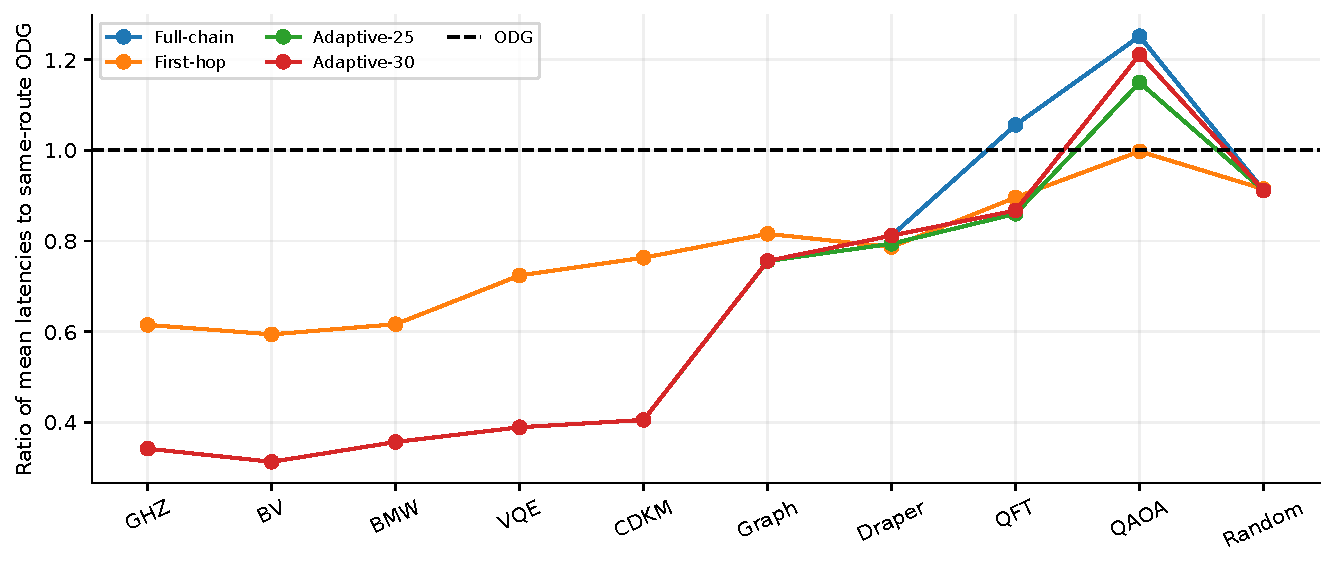
\includegraphics[width=\linewidth,height=0.37\textheight,keepaspectratio]{figures/generalisation_xy.pdf}\captionof{figure}{Ratios of seed means, three physics seeds per policy. Workload categories have no continuous order. Ratios have no confidence intervals here.}\end{center}

\begin{center}\small
\begin{longtable}{lrrrr}
\caption{Exact latency ratios plotted above; values below one favour the listed Dynamic policy.}\\
\toprule
Workload & Full-chain & First-hop & Adaptive-25 & Adaptive-30 \\
\midrule\endfirsthead
\toprule
Workload & Full-chain & First-hop & Adaptive-25 & Adaptive-30 \\
\midrule\endhead
GHZ & 0.3419 & 0.6150 & 0.3419 & 0.3419 \\
BV & 0.3130 & 0.5940 & 0.3130 & 0.3130 \\
BMW & 0.3567 & 0.6165 & 0.3567 & 0.3567 \\
VQE & 0.3891 & 0.7239 & 0.3891 & 0.3891 \\
CDKM & 0.4053 & 0.7630 & 0.4053 & 0.4053 \\
Graph & 0.7560 & 0.8158 & 0.7557 & 0.7560 \\
Draper & 0.8119 & 0.7867 & 0.7939 & 0.8119 \\
QFT & 1.0561 & 0.8961 & 0.8601 & 0.8674 \\
QAOA & 1.2516 & 0.9977 & 1.1495 & 1.2111 \\
Random & 0.9116 & 0.9146 & 0.9115 & 0.9116 \\
\bottomrule\end{longtable}\end{center}
{\footnotesize \href{https://github.com/sanjeevkrishnaa/Compiler-Driven-ACE/blob/codex/ace-scheduler-correctness/docs/latex/oct25_pre_golden/data/generalisation.csv}{Complete CSV: generalisation}. }

\begin{center}\small
\begin{longtable}{lrrrrr}
\caption{Latency (ms), mean $\pm$ SD across three seeds.}\\
\toprule
Workload & ODG & Full-chain & First-hop & Adaptive-25 & Adaptive-30 \\
\midrule\endfirsthead
\toprule
Workload & ODG & Full-chain & First-hop & Adaptive-25 & Adaptive-30 \\
\midrule\endhead
GHZ & $1.353 \pm 0.148$ & $0.463 \pm 0.000$ & $0.832 \pm 0.106$ & $0.463 \pm 0.000$ & $0.463 \pm 0.000$ \\
BV & $1.419 \pm 0.140$ & $0.444 \pm 0.000$ & $0.843 \pm 0.083$ & $0.444 \pm 0.000$ & $0.444 \pm 0.000$ \\
BMW & $1.268 \pm 0.039$ & $0.452 \pm 0.004$ & $0.782 \pm 0.017$ & $0.452 \pm 0.004$ & $0.452 \pm 0.004$ \\
VQE & $1.298 \pm 0.039$ & $0.505 \pm 0.021$ & $0.940 \pm 0.033$ & $0.505 \pm 0.021$ & $0.505 \pm 0.021$ \\
CDKM & $1.349 \pm 0.025$ & $0.547 \pm 0.009$ & $1.030 \pm 0.032$ & $0.547 \pm 0.009$ & $0.547 \pm 0.009$ \\
Graph & $1.431 \pm 0.093$ & $1.082 \pm 0.090$ & $1.168 \pm 0.043$ & $1.082 \pm 0.177$ & $1.082 \pm 0.090$ \\
Draper & $1.342 \pm 0.013$ & $1.090 \pm 0.033$ & $1.056 \pm 0.021$ & $1.066 \pm 0.062$ & $1.090 \pm 0.033$ \\
QFT & $1.383 \pm 0.016$ & $1.461 \pm 0.198$ & $1.240 \pm 0.050$ & $1.190 \pm 0.034$ & $1.200 \pm 0.055$ \\
QAOA & $1.345 \pm 0.014$ & $1.683 \pm 0.040$ & $1.342 \pm 0.091$ & $1.546 \pm 0.128$ & $1.629 \pm 0.110$ \\
Random & $1.312 \pm 0.005$ & $1.196 \pm 0.005$ & $1.200 \pm 0.003$ & $1.196 \pm 0.009$ & $1.196 \pm 0.005$ \\
\bottomrule\end{longtable}\end{center}
{\footnotesize \href{https://github.com/sanjeevkrishnaa/Compiler-Driven-ACE/blob/codex/ace-scheduler-correctness/docs/latex/oct25_pre_golden/data/generalisation.csv}{Complete CSV: generalisation}. }

\begin{center}\small
\begin{longtable}{lrrrrr}
\caption{Makespan (s), mean $\pm$ SD across three seeds.}\\
\toprule
Workload & ODG & Full-chain & First-hop & Adaptive-25 & Adaptive-30 \\
\midrule\endfirsthead
\toprule
Workload & ODG & Full-chain & First-hop & Adaptive-25 & Adaptive-30 \\
\midrule\endhead
GHZ & $0.202 \pm 0.004$ & $0.181 \pm 0.000$ & $0.190 \pm 0.003$ & $0.181 \pm 0.000$ & $0.181 \pm 0.000$ \\
BV & $0.760 \pm 0.003$ & $0.736 \pm 0.000$ & $0.746 \pm 0.002$ & $0.736 \pm 0.000$ & $0.736 \pm 0.000$ \\
BMW & $6.213 \pm 0.006$ & $6.095 \pm 0.001$ & $6.143 \pm 0.002$ & $6.095 \pm 0.001$ & $6.095 \pm 0.001$ \\
VQE & $0.337 \pm 0.006$ & $0.273 \pm 0.001$ & $0.314 \pm 0.004$ & $0.273 \pm 0.001$ & $0.273 \pm 0.001$ \\
CDKM & $3.371 \pm 0.013$ & $3.008 \pm 0.003$ & $3.227 \pm 0.015$ & $3.008 \pm 0.003$ & $3.008 \pm 0.003$ \\
Graph & $0.128 \pm 0.003$ & $0.113 \pm 0.003$ & $0.122 \pm 0.004$ & $0.114 \pm 0.005$ & $0.113 \pm 0.003$ \\
Draper & $2.389 \pm 0.015$ & $2.176 \pm 0.009$ & $2.262 \pm 0.023$ & $2.163 \pm 0.032$ & $2.176 \pm 0.009$ \\
QFT & $2.101 \pm 0.028$ & $2.005 \pm 0.060$ & $2.050 \pm 0.037$ & $1.980 \pm 0.035$ & $1.955 \pm 0.033$ \\
QAOA & $2.056 \pm 0.026$ & $2.139 \pm 0.009$ & $2.045 \pm 0.050$ & $2.082 \pm 0.062$ & $2.109 \pm 0.057$ \\
Random & $15.043 \pm 0.082$ & $13.514 \pm 0.072$ & $14.085 \pm 0.007$ & $13.535 \pm 0.043$ & $13.514 \pm 0.072$ \\
\bottomrule\end{longtable}\end{center}
{\footnotesize \href{https://github.com/sanjeevkrishnaa/Compiler-Driven-ACE/blob/codex/ace-scheduler-correctness/docs/latex/oct25_pre_golden/data/generalisation.csv}{Complete CSV: generalisation}. }

\begin{center}\small
\begin{longtable}{lrrrrr}
\caption{Delivered fidelity, mean $\pm$ SD across three seeds.}\\
\toprule
Workload & ODG & Full-chain & First-hop & Adaptive-25 & Adaptive-30 \\
\midrule\endfirsthead
\toprule
Workload & ODG & Full-chain & First-hop & Adaptive-25 & Adaptive-30 \\
\midrule\endhead
GHZ & $0.9498 \pm 0.0000$ & $0.9416 \pm 0.0003$ & $0.9450 \pm 0.0001$ & $0.9416 \pm 0.0003$ & $0.9416 \pm 0.0003$ \\
BV & $0.9498 \pm 0.0000$ & $0.9418 \pm 0.0003$ & $0.9449 \pm 0.0001$ & $0.9418 \pm 0.0003$ & $0.9418 \pm 0.0003$ \\
BMW & $0.9498 \pm 0.0000$ & $0.9414 \pm 0.0001$ & $0.9449 \pm 0.0001$ & $0.9414 \pm 0.0001$ & $0.9414 \pm 0.0001$ \\
VQE & $0.9498 \pm 0.0000$ & $0.9417 \pm 0.0002$ & $0.9460 \pm 0.0001$ & $0.9417 \pm 0.0002$ & $0.9417 \pm 0.0002$ \\
CDKM & $0.9498 \pm 0.0000$ & $0.9430 \pm 0.0001$ & $0.9475 \pm 0.0001$ & $0.9430 \pm 0.0001$ & $0.9430 \pm 0.0001$ \\
Graph & $0.9498 \pm 0.0000$ & $0.9451 \pm 0.0007$ & $0.9486 \pm 0.0001$ & $0.9458 \pm 0.0008$ & $0.9451 \pm 0.0007$ \\
Draper & $0.9498 \pm 0.0000$ & $0.9443 \pm 0.0004$ & $0.9469 \pm 0.0001$ & $0.9441 \pm 0.0005$ & $0.9443 \pm 0.0004$ \\
QFT & $0.9498 \pm 0.0000$ & $0.9443 \pm 0.0001$ & $0.9480 \pm 0.0000$ & $0.9473 \pm 0.0000$ & $0.9466 \pm 0.0000$ \\
QAOA & $0.9498 \pm 0.0000$ & $0.9459 \pm 0.0004$ & $0.9479 \pm 0.0001$ & $0.9467 \pm 0.0004$ & $0.9463 \pm 0.0003$ \\
Random & $0.9498 \pm 0.0000$ & $0.9468 \pm 0.0000$ & $0.9482 \pm 0.0001$ & $0.9469 \pm 0.0001$ & $0.9468 \pm 0.0000$ \\
\bottomrule\end{longtable}\end{center}
{\footnotesize \href{https://github.com/sanjeevkrishnaa/Compiler-Driven-ACE/blob/codex/ace-scheduler-correctness/docs/latex/oct25_pre_golden/data/generalisation.csv}{Complete CSV: generalisation}. }

\begin{center}\small
\begin{longtable}{lrrrrr}
\caption{Readiness fraction, mean $\pm$ SD across three seeds.}\\
\toprule
Workload & ODG & Full-chain & First-hop & Adaptive-25 & Adaptive-30 \\
\midrule\endfirsthead
\toprule
Workload & ODG & Full-chain & First-hop & Adaptive-25 & Adaptive-30 \\
\midrule\endhead
GHZ & $0.000 \pm 0.000$ & $1.000 \pm 0.000$ & $0.625 \pm 0.000$ & $1.000 \pm 0.000$ & $1.000 \pm 0.000$ \\
BV & $0.000 \pm 0.000$ & $1.000 \pm 0.000$ & $0.640 \pm 0.000$ & $1.000 \pm 0.000$ & $1.000 \pm 0.000$ \\
BMW & $0.000 \pm 0.000$ & $0.998 \pm 0.004$ & $0.625 \pm 0.000$ & $0.998 \pm 0.004$ & $0.998 \pm 0.004$ \\
VQE & $0.000 \pm 0.000$ & $0.974 \pm 0.006$ & $0.471 \pm 0.000$ & $0.974 \pm 0.006$ & $0.974 \pm 0.006$ \\
CDKM & $0.000 \pm 0.000$ & $0.868 \pm 0.021$ & $0.330 \pm 0.008$ & $0.868 \pm 0.021$ & $0.868 \pm 0.021$ \\
Graph & $0.000 \pm 0.000$ & $0.645 \pm 0.023$ & $0.224 \pm 0.026$ & $0.522 \pm 0.040$ & $0.645 \pm 0.023$ \\
Draper & $0.000 \pm 0.000$ & $0.597 \pm 0.047$ & $0.367 \pm 0.002$ & $0.619 \pm 0.053$ & $0.597 \pm 0.047$ \\
QFT & $0.000 \pm 0.000$ & $0.518 \pm 0.036$ & $0.238 \pm 0.002$ & $0.310 \pm 0.005$ & $0.371 \pm 0.007$ \\
QAOA & $0.000 \pm 0.000$ & $0.369 \pm 0.030$ & $0.235 \pm 0.008$ & $0.318 \pm 0.035$ & $0.347 \pm 0.030$ \\
Random & $0.000 \pm 0.000$ & $0.341 \pm 0.003$ & $0.232 \pm 0.009$ & $0.336 \pm 0.009$ & $0.341 \pm 0.003$ \\
\bottomrule\end{longtable}\end{center}
{\footnotesize \href{https://github.com/sanjeevkrishnaa/Compiler-Driven-ACE/blob/codex/ace-scheduler-correctness/docs/latex/oct25_pre_golden/data/generalisation.csv}{Complete CSV: generalisation}. }

\begin{center}\small
\begin{longtable}{lrrrrr}
\caption{Compiler waste (percent), mean $\pm$ SD across three seeds.}\\
\toprule
Workload & ODG & Full-chain & First-hop & Adaptive-25 & Adaptive-30 \\
\midrule\endfirsthead
\toprule
Workload & ODG & Full-chain & First-hop & Adaptive-25 & Adaptive-30 \\
\midrule\endhead
GHZ & n/a & $0.000 \pm 0.000$ & $0.000 \pm 0.000$ & $0.000 \pm 0.000$ & $0.000 \pm 0.000$ \\
BV & n/a & $0.000 \pm 0.000$ & $0.000 \pm 0.000$ & $0.000 \pm 0.000$ & $0.000 \pm 0.000$ \\
BMW & n/a & $0.231 \pm 0.401$ & $0.000 \pm 0.000$ & $0.231 \pm 0.401$ & $0.231 \pm 0.401$ \\
VQE & n/a & $0.971 \pm 0.971$ & $0.000 \pm 0.000$ & $0.971 \pm 0.971$ & $0.971 \pm 0.971$ \\
CDKM & n/a & $1.305 \pm 0.814$ & $2.123 \pm 1.603$ & $1.305 \pm 0.814$ & $1.305 \pm 0.814$ \\
Graph & n/a & $4.774 \pm 2.776$ & $5.000 \pm 5.000$ & $4.317 \pm 4.348$ & $4.774 \pm 2.776$ \\
Draper & n/a & $1.147 \pm 0.519$ & $0.276 \pm 0.120$ & $0.942 \pm 0.455$ & $1.147 \pm 0.519$ \\
QFT & n/a & $0.902 \pm 0.173$ & $1.450 \pm 0.176$ & $1.450 \pm 0.203$ & $1.114 \pm 0.235$ \\
QAOA & n/a & $1.930 \pm 0.662$ & $1.171 \pm 0.152$ & $1.539 \pm 0.529$ & $1.791 \pm 0.481$ \\
Random & n/a & $3.876 \pm 0.021$ & $4.336 \pm 0.536$ & $3.955 \pm 0.152$ & $3.876 \pm 0.021$ \\
\bottomrule\end{longtable}\end{center}
{\footnotesize \href{https://github.com/sanjeevkrishnaa/Compiler-Driven-ACE/blob/codex/ace-scheduler-correctness/docs/latex/oct25_pre_golden/data/generalisation.csv}{Complete CSV: generalisation}. }


\section{The generalisation lesson}
Sparse workloads can exploit full-chain pre-generation with little contention; first-hop-only discards useful opportunities. Dense or locally busy workloads can benefit from filtering later hops. Total migration count alone is not a sufficient classifier: graphstate is an explicit reminder that a small total count can still contain concentrated activity. Earlier worklog prose that grouped graphstate among high-volume workloads is inconsistent with its recorded 28 migrations and is not carried into this report.

Thresholds 25--30 retain full-chain outcomes on several sparse workloads and improve QFT-48. On QAOA they remain worse than first-hop-only. The random-circuit result is not improved by these thresholds. The data supports conditional adaptation as a promising direction, rather than one fixed rule being best everywhere. The mechanism should be checked per workload before turning this observation into a general law.

\chapter{Mapping comparison, extra controls and implementation status}
\section{HQA versus T-HQA is a separate experiment}
The main QFT-96 routing study holds the \emph{historical reconstructed placement} fixed. It was not retroactively rerun with the newly selected T-HQA placement. A separate mapper-only comparison used QFT-96, OEE initial placement, eight mapper qubit slots per core, two initially reserved slots per core, a $4\times4$ mesh and reliability seeds 42--44.
\begin{center}\small
\begin{longtable}{lrrrrr}
\caption{Mapper-only HQA/T-HQA comparison. Reliability seeds are not independent placement samples.}\\
\toprule
Seed & Placer & Migrations & Hops & Mapper cost & Residual \\
\midrule\endfirsthead
\toprule
Seed & Placer & Migrations & Hops & Mapper cost & Residual \\
\midrule\endhead
42 & HQA & 1770 & 4954 & 52966.06 & 0 \\
42 & T-HQA & 1965 & 3876 & 34900.40 & 0 \\
43 & HQA & 1770 & 4954 & 19953.57 & 0 \\
43 & T-HQA & 1965 & 3876 & 20085.10 & 0 \\
44 & HQA & 1770 & 4954 & 28825.80 & 0 \\
44 & T-HQA & 1965 & 3876 & 19105.14 & 0 \\
\bottomrule\end{longtable}\end{center}
{\footnotesize \href{https://github.com/sanjeevkrishnaa/Compiler-Driven-ACE/blob/codex/ace-scheduler-correctness/docs/latex/oct25_pre_golden/data/mapper.csv}{Complete CSV: mapper}. }

T-HQA produces 3,876 exported hops versus HQA's 4,954, a reduction of 1,078 or $21.76\%$. Its reliability-weighted cost is not uniformly better across seeds. Mapper cost, path-quality sum and EPR-latency proxy are mapper objectives, not measured ACE arrival-to-delivery latency. No claim that T-HQA has already reduced physical ACE latency follows from this table alone.

\section{Controls implemented before the boundary}
The last included commit \commit{4aa3345} adds planner lead, predecessor distance and a chain-depth interface. The predecessor-distance control generalises a trigger from the immediate previous hop to an earlier hop in the chain. Planner lead changes how far before the target layer planning starts searching. These controls expand the available design space, but this snapshot has no separately archived result matrix demonstrating their sweep. They are documented as implemented, not reported as validated performance gains.

\section{Code and verification provenance}
The mapper implementation is a dependency; the adapter, placement contract, explicit routing exporters and comparison tools are project work. The relevant modified ACE integration points are \texttt{compiler\_trace.py}, \texttt{compiler\_scheduler.py}, \texttt{parallel\_core.py}, \texttt{request\_scheduler.py} and \texttt{run\_trace\_comparison.py}. The source ledger identifies exact Git blobs for all consumed evidence.

Historical verification scripts independently parsed routes, checked endpoints and adjacency, rederived touch loads and checked statistics. The adaptive verification tested full-chain/default equivalence, large-threshold equivalence, threshold-zero/first-hop equivalence and allowed later-hop preparations. Those historical checks support the implementation record; this report's new validation specifically checks the stored observations and control regression. It does not claim to rerun every simulator test or every experiment.

\chapter{Conclusions, limitations and next research questions}
The strongest supported result is that changing the pattern of shared-memory use matters as much as reducing EPR generation time. At four memories per core, full-chain Dynamic can lose on fair request latency. XY/YX routing lowers concentrated relay demand. First-hop-only reduces later-hop occupancy. A layer-activity filter combines full-chain preparation in quiet layers with conservative preparation in busy ones and produces the lowest mean latency among the four policies in the 30-seed XY confirmation.

The result is $1.175$ ms for threshold-25 Dynamic against $1.340$ ms for XY ODG, with makespans approximately $3.992$ s and $4.244$ s. The gain is conditional on the fixed placement, routing, memory budget, physical model and evaluation protocol. Fidelity, waste and the sparse-workload trade-offs remain part of the result, not footnotes to discard.

Three limitations should guide interpretation. First, QFT-96's original reliability map is absent, so reliability-aware alternatives are reconstructed-map experiments. Second, the ten-workload generalisation corpus is 48-qubit and uses only three physics seeds. Third, adjacent-hop EPR delivery omits data-qubit relay occupancy, full teleportation/gate execution and final algorithm fidelity. These omissions limit claims about full distributed QFT runtime and hardware feasibility.

The immediate research questions are whether an adaptive signal can be scaled by capacity and local demand, whether freed planner resources should be replanned, and whether the improvement survives physical coherence/control-delay changes and independent placements. The golden study was started to systematise such questions. Its results belong in a separate report and do not retroactively strengthen the October 25 evidence.

\appendix
\chapter{Commit-by-commit research record}
The following commits are ancestors of the pre-golden snapshot after the handoff \texttt{1cc7eb6}. Links resolve to immutable commits. The list follows Git ancestry order; author timestamps need not follow the logical sequence.
\begin{longtable}{p{.15\linewidth}p{.77\linewidth}}\toprule Commit & Recorded change\\\midrule\endhead
\href{https://github.com/sanjeevkrishnaa/Compiler-Driven-ACE/commit/2a6b73a1c232912a54d5a5254312461526473c14}{2a6b73a} & [forwarding] - Relayed classical messages keep their original sender (multi-hop swapping completes) \\
\href{https://github.com/sanjeevkrishnaa/Compiler-Driven-ACE/commit/49da2d1aef1021c3bada3097b96b32dcce172355}{49da2d1} & [worklog] - Work log for 2026-10-25: 96-qubit model, swapping decision, ACE runs, ACE paper notes \\
\href{https://github.com/sanjeevkrishnaa/Compiler-Driven-ACE/commit/2cb86d664950c4c1757d50d931b462f6faa60814}{2cb86d6} & [metrics] - Measure compiler latency from request arrival through completion \\
\href{https://github.com/sanjeevkrishnaa/Compiler-Driven-ACE/commit/6af687f2c80906a693f3da56bd2f3b2849a33111}{6af687f} & [timing] - Derive reservation starts from RSVP control delay \\
\href{https://github.com/sanjeevkrishnaa/Compiler-Driven-ACE/commit/34f6a05ed922a45420f3aa31a599f4cd601acf29}{34f6a05} & [metrics] Headline latency without the lead subtraction, plus median/p95/max and cache storage time \\
\href{https://github.com/sanjeevkrishnaa/Compiler-Driven-ACE/commit/e2b418afa7e5c01164d66222ff356167f4327a8d}{e2b418a} & [experiments] - Record QFT-96 timing-model matrix \\
\href{https://github.com/sanjeevkrishnaa/Compiler-Driven-ACE/commit/ffbc571373919dcea3cbe11a118a2eecc19ffbcd}{ffbc571} & [merge] - Integrate corrected timing and QFT-96 experiments \\
\href{https://github.com/sanjeevkrishnaa/Compiler-Driven-ACE/commit/447aa3c90a1966f5e192e2fd735286c8ab3a30bf}{447aa3c} & [mapping] Add auditable migration trace and explicit routing boundary \\
\href{https://github.com/sanjeevkrishnaa/Compiler-Driven-ACE/commit/e78c962e9498163a1b252d5e8e2f187252a6157b}{e78c962} & [research] Record ACE timing provenance and metric contract \\
\href{https://github.com/sanjeevkrishnaa/Compiler-Driven-ACE/commit/b700f55a3fe430a7b0c9232d1c45da114b5b44ea}{b700f55} & [mapping] Add reproducible placement export command and manifest \\
\href{https://github.com/sanjeevkrishnaa/Compiler-Driven-ACE/commit/310dd441b739742c44a77f8cbae4b19c0ec5a23b}{310dd44} & [experiments] Reproduce QFT-96 physical timing with 30 per-qubit seeds \\
\href{https://github.com/sanjeevkrishnaa/Compiler-Driven-ACE/commit/3dfd01314512778b1f67e85775215a45faf6b9c1}{3dfd013} & [mapping] Import legacy hop traces into validated migrations \\
\href{https://github.com/sanjeevkrishnaa/Compiler-Driven-ACE/commit/9c9d561e45bba7286048f76516a1ed0038cea947}{9c9d561} & [visualization] Add QFT-96 latency and makespan figures \\
\href{https://github.com/sanjeevkrishnaa/Compiler-Driven-ACE/commit/07a7064f356cef5037d688f69d8cf8617e0020ef}{07a7064} & [mapping] Export placement contracts and validated QFT-96 routing traces \\
\href{https://github.com/sanjeevkrishnaa/Compiler-Driven-ACE/commit/351541166c28a9be0abc1939bbd0efbf5b229e40}{3515411} & [research] Add post-mapping plan, routing comparison, and Dynamic sweep tooling \\
\href{https://github.com/sanjeevkrishnaa/Compiler-Driven-ACE/commit/3582898432a1310be1ebe8008eb33b5a5e768c01}{3582898} & [routing] Record QFT-96 routing results and add preparation-trigger policies \\
\href{https://github.com/sanjeevkrishnaa/Compiler-Driven-ACE/commit/189220b446fc2b987750ebeb792ff81d6762958b}{189220b} & [routing] Add pre-registered XY mechanism tests and controlled route interventions \\
\href{https://github.com/sanjeevkrishnaa/Compiler-Driven-ACE/commit/75414b396996ed89c5f14b75b12f751107fa6ace}{75414b3} & [dynamic] Screen launch policies and add per-core wait diagnostics \\
\href{https://github.com/sanjeevkrishnaa/Compiler-Driven-ACE/commit/e2d4a9ac58aeefdcbcb9c246b3b6fdfe028520a2}{e2d4a9a} & [routing] Preserve declared empty layers in intervention traces \\
\href{https://github.com/sanjeevkrishnaa/Compiler-Driven-ACE/commit/d2f3253de2531e067924a560e031c5f5758e584b}{d2f3253} & [verification] Independently verify routes, loads, waits, and statistics \\
\href{https://github.com/sanjeevkrishnaa/Compiler-Driven-ACE/commit/e830992ed9cbd286d7e8072bbf5c9adff8e7283a}{e830992} & [overnight-batch] - Queue remaining first-hop-only confirmation, parameter grid and ten-benchmark generalisation runs \\
\href{https://github.com/sanjeevkrishnaa/Compiler-Driven-ACE/commit/3a68bba5cec3fdb8d29d3c00daed96e137613d05}{3a68bba} & [why-xy-wins] - Mechanism confirmed (static excess predicts ODG wait, Spearman 0.90-0.96); first-hop-only generalisation test shows it is a trade, not a universal win \\
\href{https://github.com/sanjeevkrishnaa/Compiler-Driven-ACE/commit/5a980259a49db034736279437c9b8aeed279d31a}{5a98025} & [verification] - Fixes found in pass-2 review (core count from trace header, makespan label); overnight batch and why-XY results on disk \\
\href{https://github.com/sanjeevkrishnaa/Compiler-Driven-ACE/commit/1da2711d92c065428d2a387532e64a10aebb508f}{1da2711} & [dynamic-redesign] - Log congestion-adaptive pre-generation design, verification and results \\
\href{https://github.com/sanjeevkrishnaa/Compiler-Driven-ACE/commit/6c2d35e081f961ada441ee27a1839da82470d53a}{6c2d35e} & [mapping] Set T-HQA for new studies and compare it with HQA \\
\href{https://github.com/sanjeevkrishnaa/Compiler-Driven-ACE/commit/82aac5e1bdf39e380aee3894e73be7f959ea33df}{82aac5e} & [dynamic-redesign] - Congestion-adaptive preparation: prepare the full chain, drop later hops only in locally busy layers; tests and pass-2 verification \\
\href{https://github.com/sanjeevkrishnaa/Compiler-Driven-ACE/commit/0600051422853d87687ee570ac0f03b3c1a740f8}{0600051} & [dynamic-redesign] - Congestion-threshold sweep and generalisation: threshold~25-30 beats first-hop-only on QFT-96/XY and matches full-chain on sparse benchmarks \\
\href{https://github.com/sanjeevkrishnaa/Compiler-Driven-ACE/commit/4aa334542e9b9c8fe7a5f9cc8fe48ee2e4d2fa55}{4aa3345} & [dynamic-controls] Add planner lead, predecessor-distance, and chain-depth controls \\
\bottomrule\end{longtable}

\chapter{Data, source links and reproduction}
\section{Evidence package}
\begin{longtable}{p{.37\linewidth}p{.55\linewidth}}
\toprule File & Role\\\midrule\endhead
\texttt{data/per\_seed\_results.csv} & Complete imported observations, with family, cell, original source path and every archived runner column.\\
\texttt{data/all\_metrics.csv} & Mean/sample SD of the documented key metrics for every policy cell.\\
\texttt{data/source\_ledger.csv} & Git snapshot, Git blob and SHA-256 for each consumed evidence file.\\
\texttt{data/validation.json} & Result checks, row counts and recomputed mechanism correlation.\\
\texttt{data/routing.csv} & Five-route two-policy summary.\\
\texttt{data/launch\_screen.csv} & All 26 route/launch screen cells.\\
\texttt{data/routing\_mechanism.csv} & Static excess, waits and means for all 21 route arms.\\
\texttt{data/per\_core\_wait.csv} & Core-level endpoint/relay attribution used in the diagnostic figure.\\
\texttt{data/confirmation.csv} & Four-policy confirmation on supplied, XY and YX.\\
{\scriptsize\texttt{data/confirmation\_comparisons.csv}} & Ratios and exploratory unadjusted Welch comparisons to same-route ODG.\\
\texttt{data/threshold.csv} & Ten threshold settings and all documented key metrics.\\
\texttt{data/parameter\_grid.csv} & Eleven memory/admission screens.\\
\texttt{data/generalisation.csv} & All ten-workload, three-seed result cells.\\
\texttt{data/mapper.csv} & Six HQA/T-HQA mapper observations.\\
\texttt{data/commits.csv} & Immutable commit identifiers and recorded subjects.\\
\bottomrule
\end{longtable}
\href{\repo/tree/codex/ace-scheduler-correctness/docs/latex/oct25_pre_golden/data}{Browse the complete report data directory}. Derived report CSVs are committed with this report. Original result and metadata links resolve to the frozen snapshot, allowing every row to be traced to the historical evidence.

\section{Rebuild the report without rerunning experiments}
From the repository root, use a Python environment with NumPy, SciPy and Matplotlib:
\begin{verbatim}
python tools/build_oct25_report.py
cd docs/latex/oct25_pre_golden
tectonic main.tex
\end{verbatim}
The script reads Git objects, validates stored seeds/completion/control results, regenerates tables/figures and records hashes. It does not invoke ACE, mutate archived experiments or reuse golden-study data. It requires the historical snapshot to be available locally.

\section{Rerun an experiment deliberately}
To reproduce physical runs, use the archived experiment metadata and command record with matching source hashes and the matching SeQUeNCe dependency. A historical shell wrapper alone is insufficient: some wrappers embed the environment path of a sibling checkout, or skip an existing summary without checking its configuration. These risks affect a future rerun; they do not justify altering the historical observations.

\src{results/routing\_study\_2026-10-25/runs/xy/metadata.json}{Example: complete XY routing metadata};
\src{results/overnight\_2026-10-25/P2\_grid/P2\_cm3\_tm4/command.txt}{Example: exact first-hop parameter command};
\src{results/congestion\_adaptive\_confirm\_2026-10-25/xy/metadata.json}{Example: adaptive confirmation metadata}.

\section{Validation interpretation}
The new report validates unique strategy/seed observations, consistency with each file's metadata, metric version 3, complete requests and exact supplied-route control latency/makespan against the separately archived physical reference. An independent text parser also checks all 21 routed traces for adjacency, contiguous chains, placement replay, common endpoints, declared layers and expected hop counts; it rederives static excess at capacities 2, 3, 4, 6 and 8. The report recomputes every plotted mean and SD from the frozen per-seed rows. These checks establish internal traceability and arithmetic correctness of this retrospective. They do not establish 100\% physical correctness of ACE or remove the model limitations above.
\end{document}
